\newcommand{\Arbeit}{Master-Thesis}
\newcommand{\Autor}{Matthias Fey}
\newcommand{\Titel}{Convolutional Neural Networks auf Graphrepr{\"a}sentationen von Bildern}
\newcommand{\Erstgutachter}{Prof.~Dr.~Heinrich~M{\"u}ller}
\newcommand{\Zweitgutachter}{M.Sc.~Jan~Eric~Lenssen}
\newcommand{\Lehrstuhl}{Lehrstuhl Informatik VII}
\newcommand{\Lehrstuhltitel}{Graphische Systeme}
\newcommand{\Universitaet}{TU Dortmund}
\newcommand{\Fakultaet}{Fakult{\"a}t f{\"u}r Informatik}

\newcommand{\dhe}{d.h.}
\newcommand{\zB}{zum Beispiel}
\newcommand{\bzw}{bzw.}
\newcommand{\bspw}{beispielsweise}
\newcommand{\vgl}{vgl.}
\newcommand{\bzgl}{bez{\"u}glich}
\newcommand{\oBdA}{o.B.d.A.}
\newcommand{\evtl}{eventuell}
\newcommand{\gdw}{genau dann, wenn}
\newcommand{\ggf}{gegebenenfalls}
\newcommand{\engl}{engl.}

\newcommand{\ma}[1]{\ensuremath{\mathbf{#1}}}
\newcommand{\ve}[1]{\ensuremath{\mathbf{#1}}}


\documentclass[pdftex,12pt,a4paper,twoside,ngerman,numbers=noenddot]{scrbook}

% -------------------------------------------------------------------

% Seitenformat anpassen
\usepackage[a4paper,left=3.5cm,right=2.5cm,bottom=3.5cm,top=3cm]{geometry}
\setlength{\headheight}{19pt}

% -------------------------------------------------------------------

% Fix für alte Pakete mit KOMA Warnung
\usepackage{scrhack}

% -------------------------------------------------------------------

% Absolute Positionierung für Titelseite
\usepackage[absolute,overlay]{textpos}
\setlength{\TPHorizModule}{1mm}
\setlength{\TPVertModule}{\TPHorizModule}
\textblockorigin{0mm}{0mm}
\usepackage{setspace}

% -------------------------------------------------------------------

% Schrifteinstellungen
\usepackage{lmodern}
\usepackage[english,main=ngerman]{babel}
\usepackage[utf8]{inputenc}
\usepackage[T1]{fontenc}
\usepackage{ae,aecompl}

% -------------------------------------------------------------------

% Bibtex deutsch
\usepackage[numbers,sort]{natbib}

% -------------------------------------------------------------------

% Anführungszeichen
\usepackage[babel,german=quotes]{csquotes}

% -------------------------------------------------------------------

% URLs
\usepackage{url}

% Trennung langer URLs
\usepackage[hyphenbreaks]{breakurl}
\def\UrlBreaks{\do\a\do\b\do\c\do\d\do\e\do\f\do\g\do\h\do\i\do\j\do\k\do\l%
\do\m\do\n\do\o\do\p\do\q\do\r\do\s\do\t\do\u\do\v\do\w\do\x\do\y\do\z\do\0%
\do\1\do\2\do\3\do\4\do\5\do\6\do\7\do\8\do\9\do\-}%

% -------------------------------------------------------------------

% Caption anpassen
\usepackage[margin=0pt,font=small,labelfont=bf]{caption}

% -------------------------------------------------------------------

% Tabellen
\usepackage{booktabs}  % bessere Linien
\usepackage{siunitx}  % Ausrichtung von Dezimalstellen

% -------------------------------------------------------------------

% Zeilenabstand einstellen
\renewcommand{\baselinestretch}{1.25}

% Floating-Umgebungen anpassen
\renewcommand{\topfraction}{0.9}
\renewcommand{\bottomfraction}{0.8}

% -------------------------------------------------------------------

% Keine Einrücktiefe der ersten Zeile eines neuen Absatzes.
\parindent=0cm

% -------------------------------------------------------------------

% Kopfzeile hinzufügen
\usepackage[headsepline]{scrlayer-scrpage}
\clearpairofpagestyles{}

\lehead{\pagemark}
\rehead{\headmark}
\rohead{\pagemark}
\lohead{\headmark}

% -------------------------------------------------------------------

% Eigene Farben
\usepackage{xcolor}
\definecolor{TUGreen}{rgb}{0.517,0.721,0.094}
\definecolor{red}{rgb}{1,0,0}

% -------------------------------------------------------------------

% Algorithmen
\usepackage[plain,chapter]{algorithm}
\usepackage{algorithmic}

% Algorithmen anpassen
\renewcommand{\algorithmicrequire}{\textit{Eingabe:}}
\renewcommand{\algorithmicensure}{\textit{Ausgabe:}}
\floatname{algorithm}{Algorithmus}
\renewcommand{\listalgorithmname}{Algorithmenverzeichnis}
\renewcommand{\algorithmiccomment}[1]{\color{grau}{// #1}}

% -------------------------------------------------------------------

% Grafikpakete einbinden
\usepackage{graphicx}
\usepackage{subfigure}
\usepackage{pdfpages}
\usepackage{tikz}
\usetikzlibrary{decorations.pathreplacing}

% -------------------------------------------------------------------

% Mathematikpakete einbinden

\usepackage{amsmath,amssymb,amsthm}
\usepackage{mathtools}

% -------------------------------------------------------------------

% Todonotes einbinden

\usepackage{todonotes}

% -------------------------------------------------------------------

% Glossar
\usepackage[toc]{glossaries}
\glstoctrue{}
\makeglossaries{}
\newglossaryentry{N}{name=\ensuremath{\mathbb{N}}, description={Menge}}
\newglossaryentry{R}{name=\ensuremath{\mathbb{R}}, description={Menge der reellen Zahlen}}
\newglossaryentry{R+}{name=\ensuremath{\mathbb{R}^+}, description={Menge der positiven reellen Zahlen inklusive Null}}

\newglossaryentry{I}{name=\ma{I}, description={Identitätsmatrix}}

\newglossaryentry{diag}{name=\ensuremath{\mathrm{diag}}, description={Diagonalfunktion}}
\newglossaryentry{ortho}{name=\ensuremath{\perp}, description={Orthogonalität}}
\newglossaryentry{hadamard}{name=\ensuremath{\odot}, description={elementweises Hadamard-Produkt}}
\newglossaryentry{O}{name=\ensuremath{\mathcal{O}}, description={O-Notation}}
\newglossaryentry{T}{name=\ensuremath{T}, description={Tschebyschow-Polynom}}

\newglossaryentry{G}{name=\ensuremath{\mathcal{G}}, description={Graph}}
\newglossaryentry{V}{name=\ensuremath{\mathcal{V}}, description={Knotenmenge ${\left\{v_i\right\}}^N_{i=1}$ eines Graphen \gls{G}}}
\newglossaryentry{v}{name={\ensuremath{v}}, description={Knoten eines Graphen}}
\newglossaryentry{A}{name=\ma{A}, description={Adjazentmatrix eines Graphen \gls{G}}}
\newglossaryentry{D}{name=\ma{D}, description={gewichtete Gradmatrix}}
\newglossaryentry{L}{name=\ma{L}, description={Laplacian, unnormalisiert}}
\newglossaryentry{Lnorm}{name=\ma{\tilde{L}}, description={Laplacian, normalisiert}}
\newglossaryentry{Lboth}{name=\ma{\mathcal{L}}, description={Laplacian, normalisiert oder unnormalisiert}}
\newglossaryentry{w}{name=\ensuremath{w}, description={Gewichtsfunktion der Kanten eines Graph \gls{G} mit $\gls{w} \colon \gls{V} \times \gls{V} \to \gls{R+}$}}
\newglossaryentry{adj}{name=\ensuremath{\sim}, description={Adjazenzrelation zweiter Knoten eines Graphen \gls{G} mit $u \gls{adj} v$ genau dann, wenn $u$ und $v$ adjazent}}
\newglossaryentry{d}{name=\ensuremath{d}, description={gewichtete Gradfunktion der Knoten eines Graphen \gls{G} mit $\gls{d} \colon \gls{V} \to \gls{R+}$}}
\newglossaryentry{s}{name=\ensuremath{s}, description={kürzeste Pfaddistanz mit $s \colon \gls{V} \times \gls{V} \to \gls{N}$}}

\newglossaryentry{lambda}{name=\ensuremath{\lambda}, description={Eigenwert eines Eigenwertproblems $\ma{M}\ve{u} = \lambda\ve{u}$}}
\newglossaryentry{lambdamax}{name=\ensuremath{\lambda_{\max}}, description={Größter Eigenwert eines Eigenwertproblems $\ma{M}\ve{u} = \lambda\ve{u}$}}
\newglossaryentry{Lambda}{name=\ma{\Lambda}, description={Diagonalmatrix der Eigenwerte einer Matrix \ma{M} mit $\mathrm{diag}$}}
\newglossaryentry{eiv}{name=\ve{u}, description={normierter Eigenvektor zu einem Eigenwert mit $\left\|\gls{eiv}\right\|_2 = 1$}}
\newglossaryentry{Eiv}{name=\ma{U}, description={Eigenvektormatrix $\left[\ve{u}_1, \ldots, \ve{u}_N \right] \in \mathbb{R}^{N \times N}$ von $N$ Eigenvektoren $\ve{u}_i$}}
\newglossaryentry{Lambdatilde}{name=\ma{\tilde{\Lambda}}, description={reskalierte Diagonalmatrix der Eigenwerte des Laplacian}}
\newglossaryentry{Atilde}{name=\ma{\tilde{A}}, description={reskalierte Diagonalmatrix der Eigenwerte des Laplacian}}
\newglossaryentry{Dtilde}{name=\ma{\tilde{D}}, description={reskalierte Diagonalmatrix der Eigenwerte des Laplacian}}

\newacronym[plural=CNNs, longplural={Convolutional Neural Networks}]{CNN}{CNN}{Convolutional Neural Network}
\newacronym[plural=GCNs, longplural={Graph Convolutional Networks}]{GCN}{GCN}{Graph Convolutional Network}
\newacronym{SLIC}{SLIC}{Simple Linear Iterative Clustering}
\newacronym{MNIST}{MNIST}{Modified National Institute of Standards and Technology}
\newacronym{Cifar}{CIFAR}{Canadian Institute for Advanced Research}
\newacronym{Pascal}{PASCAL VOC}{Pascal Visual Object Classes}
\newacronym{SVHN}{SVHN}{Street View House Numbers}
\newacronym{PCA}{PCA}{Haptkomponentenanalyse}


% -------------------------------------------------------------------

% Fix für \left und \right Abstände
\let\oldleft\left
\let\oldright\right
\def\left#1{\mathopen{}\oldleft#1}
\def\right#1{\oldright#1\mathclose{}}

% -------------------------------------------------------------------

% Füge einen Punkt an Paragraph-Überschriften
\let\oldparagraph=\paragraph
\renewcommand\paragraph[1]{\oldparagraph{#1.}}

% -------------------------------------------------------------------

% Informationen für PDF-Dokument festlegen
\usepackage[pdfencoding=auto]{hyperref}

\hypersetup{pdfauthor={\Autor},
            pdftitle={\Titel},
            pdfsubject={\Arbeit, \Universitaet, \Fakultaet},
            pdfproducer={LaTeX},
            pdfview=FitV,
            pdfstartview=FitV,
            pdfhighlight=/I,
            pdfborder=0 0 0,
            colorlinks=false,
            bookmarksopen,
            bookmarksopenlevel=1,
            bookmarksnumbered=false,
            plainpages=false
}


\begin{document}

% -------------------------------------------------------------------

% Titelseite
\pagestyle{empty}
\pagenumbering{alpha}

\begin{titlepage}

\definecolor{TUGreen}{rgb}{0.517,0.721,0.094}

\setlength{\TPHorizModule}{1cm}
\setlength{\TPVertModule}{1cm}
\setlength{\parindent}{0cm}

\sffamily

\vspace*{2cm}

\begin{textblock}{9}(3,5.3)
  \Large
  \begin{minipage}[c][9cm]{9cm}
    \begin{center}
      {\Huge Master-Thesis}\\
      \vspace*{1cm}
      {\huge Anwendbarkeit neuronaler Netze auf Graphrepräsentationen von Bildern}\\
      \vspace*{1cm}
      Matthias~Fey\\
      \today
    \end{center}
  \end{minipage}
  \normalsize
\end{textblock}

\begin{textblock}{9}(3,1)
  
\includegraphics[height=1.4cm]{images/tud_logo}
\end{textblock}

\begin{textblock}{15}(3,3.7)
  
\includegraphics[height=0.65cm]{images/fi_text}
\end{textblock}

\begin{textblock}{9}(3,26.5)
  
\includegraphics[height=1.2cm]{images/fi_logo}
\end{textblock}

\begin{textblock}{9}(3,20)
  \Large
  \textbf{Gutachter:}\\
  Prof.~Dr.~Heinrich~Müller\\
  M.Sc.~Jan~Eric~Lenssen
  \normalsize
\end{textblock}

\begin{textblock}{9}(3,24)
  \large
  \textcolor{TUGreen}{
    Lehrstuhl Informatik VII\\
    Graphische Systeme\\
    TU Dortmund
  }
  \normalsize
\end{textblock}

\end{titlepage}

\null{}

% -------------------------------------------------------------------

% Inhaltsverzeichnis
\pagestyle{empty}
\pagenumbering{roman}

\tableofcontents

% -------------------------------------------------------------------

% Kapitel
\cleardoublepage{}
\pagestyle{headings}
\pagenumbering{arabic}

\documentclass[pdftex,12pt,a4paper,twoside,ngerman,numbers=noenddot]{scrbook}

% -------------------------------------------------------------------

% Seitenformat anpassen
\usepackage[a4paper,left=3.5cm,right=2.5cm,bottom=3.5cm,top=3cm]{geometry}
\setlength{\headheight}{19pt}

% -------------------------------------------------------------------

% Fix für alte Pakete mit KOMA Warnung
\usepackage{scrhack}

% -------------------------------------------------------------------

% Absolute Positionierung für Titelseite
\usepackage[absolute,overlay]{textpos}
\setlength{\TPHorizModule}{1mm}
\setlength{\TPVertModule}{\TPHorizModule}
\textblockorigin{0mm}{0mm}
\usepackage{setspace}

% -------------------------------------------------------------------

% Schrifteinstellungen
\usepackage{lmodern}
\usepackage[english,main=ngerman]{babel}
\usepackage[utf8]{inputenc}
\usepackage[T1]{fontenc}
\usepackage{ae,aecompl}

% -------------------------------------------------------------------

% Bibtex deutsch
\usepackage[numbers,sort]{natbib}

% -------------------------------------------------------------------

% Anführungszeichen
\usepackage[babel,german=quotes]{csquotes}

% -------------------------------------------------------------------

% URLs
\usepackage{url}

% Trennung langer URLs
\usepackage[hyphenbreaks]{breakurl}
\def\UrlBreaks{\do\a\do\b\do\c\do\d\do\e\do\f\do\g\do\h\do\i\do\j\do\k\do\l%
\do\m\do\n\do\o\do\p\do\q\do\r\do\s\do\t\do\u\do\v\do\w\do\x\do\y\do\z\do\0%
\do\1\do\2\do\3\do\4\do\5\do\6\do\7\do\8\do\9\do\-}%

% -------------------------------------------------------------------

% Caption anpassen
\usepackage[margin=0pt,font=small,labelfont=bf]{caption}

% -------------------------------------------------------------------

% Tabellen
\usepackage{booktabs}  % bessere Linien
\usepackage{siunitx}  % Ausrichtung von Dezimalstellen

% -------------------------------------------------------------------

% Zeilenabstand einstellen
\renewcommand{\baselinestretch}{1.25}

% Floating-Umgebungen anpassen
\renewcommand{\topfraction}{0.9}
\renewcommand{\bottomfraction}{0.8}

% -------------------------------------------------------------------

% Keine Einrücktiefe der ersten Zeile eines neuen Absatzes.
\parindent=0cm

% -------------------------------------------------------------------

% Kopfzeile hinzufügen
\usepackage[headsepline]{scrlayer-scrpage}
\clearpairofpagestyles{}

\lehead{\pagemark}
\rehead{\headmark}
\rohead{\pagemark}
\lohead{\headmark}

% -------------------------------------------------------------------

% Eigene Farben
\usepackage{xcolor}
\definecolor{TUGreen}{rgb}{0.517,0.721,0.094}
\definecolor{red}{rgb}{1,0,0}

% -------------------------------------------------------------------

% Algorithmen
\usepackage[plain,chapter]{algorithm}
\usepackage{algorithmic}

% Algorithmen anpassen
\renewcommand{\algorithmicrequire}{\textit{Eingabe:}}
\renewcommand{\algorithmicensure}{\textit{Ausgabe:}}
\floatname{algorithm}{Algorithmus}
\renewcommand{\listalgorithmname}{Algorithmenverzeichnis}
\renewcommand{\algorithmiccomment}[1]{\color{grau}{// #1}}

% -------------------------------------------------------------------

% Grafikpakete einbinden
\usepackage{graphicx}
\usepackage{subfigure}
\usepackage{pdfpages}
\usepackage{tikz}
\usetikzlibrary{decorations.pathreplacing}

% -------------------------------------------------------------------

% Mathematikpakete einbinden

\usepackage{amsmath,amssymb,amsthm}
\usepackage{mathtools}

% -------------------------------------------------------------------

% Todonotes einbinden

\usepackage{todonotes}

% -------------------------------------------------------------------

% Glossar
\usepackage[toc]{glossaries}
\glstoctrue{}
\makeglossaries{}
\newglossaryentry{N}{name=\ensuremath{\mathbb{N}}, description={Menge}}
\newglossaryentry{R}{name=\ensuremath{\mathbb{R}}, description={Menge der reellen Zahlen}}
\newglossaryentry{R+}{name=\ensuremath{\mathbb{R}^+}, description={Menge der positiven reellen Zahlen inklusive Null}}

\newglossaryentry{I}{name=\ma{I}, description={Identitätsmatrix}}

\newglossaryentry{diag}{name=\ensuremath{\mathrm{diag}}, description={Diagonalfunktion}}
\newglossaryentry{ortho}{name=\ensuremath{\perp}, description={Orthogonalität}}
\newglossaryentry{hadamard}{name=\ensuremath{\odot}, description={elementweises Hadamard-Produkt}}
\newglossaryentry{O}{name=\ensuremath{\mathcal{O}}, description={O-Notation}}
\newglossaryentry{T}{name=\ensuremath{T}, description={Tschebyschow-Polynom}}

\newglossaryentry{G}{name=\ensuremath{\mathcal{G}}, description={Graph}}
\newglossaryentry{V}{name=\ensuremath{\mathcal{V}}, description={Knotenmenge ${\left\{v_i\right\}}^N_{i=1}$ eines Graphen \gls{G}}}
\newglossaryentry{v}{name={\ensuremath{v}}, description={Knoten eines Graphen}}
\newglossaryentry{A}{name=\ma{A}, description={Adjazentmatrix eines Graphen \gls{G}}}
\newglossaryentry{D}{name=\ma{D}, description={gewichtete Gradmatrix}}
\newglossaryentry{L}{name=\ma{L}, description={Laplacian, unnormalisiert}}
\newglossaryentry{Lnorm}{name=\ma{\tilde{L}}, description={Laplacian, normalisiert}}
\newglossaryentry{Lboth}{name=\ma{\mathcal{L}}, description={Laplacian, normalisiert oder unnormalisiert}}
\newglossaryentry{w}{name=\ensuremath{w}, description={Gewichtsfunktion der Kanten eines Graph \gls{G} mit $\gls{w} \colon \gls{V} \times \gls{V} \to \gls{R+}$}}
\newglossaryentry{adj}{name=\ensuremath{\sim}, description={Adjazenzrelation zweiter Knoten eines Graphen \gls{G} mit $u \gls{adj} v$ genau dann, wenn $u$ und $v$ adjazent}}
\newglossaryentry{d}{name=\ensuremath{d}, description={gewichtete Gradfunktion der Knoten eines Graphen \gls{G} mit $\gls{d} \colon \gls{V} \to \gls{R+}$}}
\newglossaryentry{s}{name=\ensuremath{s}, description={kürzeste Pfaddistanz mit $s \colon \gls{V} \times \gls{V} \to \gls{N}$}}

\newglossaryentry{lambda}{name=\ensuremath{\lambda}, description={Eigenwert eines Eigenwertproblems $\ma{M}\ve{u} = \lambda\ve{u}$}}
\newglossaryentry{lambdamax}{name=\ensuremath{\lambda_{\max}}, description={Größter Eigenwert eines Eigenwertproblems $\ma{M}\ve{u} = \lambda\ve{u}$}}
\newglossaryentry{Lambda}{name=\ma{\Lambda}, description={Diagonalmatrix der Eigenwerte einer Matrix \ma{M} mit $\mathrm{diag}$}}
\newglossaryentry{eiv}{name=\ve{u}, description={normierter Eigenvektor zu einem Eigenwert mit $\left\|\gls{eiv}\right\|_2 = 1$}}
\newglossaryentry{Eiv}{name=\ma{U}, description={Eigenvektormatrix $\left[\ve{u}_1, \ldots, \ve{u}_N \right] \in \mathbb{R}^{N \times N}$ von $N$ Eigenvektoren $\ve{u}_i$}}
\newglossaryentry{Lambdatilde}{name=\ma{\tilde{\Lambda}}, description={reskalierte Diagonalmatrix der Eigenwerte des Laplacian}}
\newglossaryentry{Atilde}{name=\ma{\tilde{A}}, description={reskalierte Diagonalmatrix der Eigenwerte des Laplacian}}
\newglossaryentry{Dtilde}{name=\ma{\tilde{D}}, description={reskalierte Diagonalmatrix der Eigenwerte des Laplacian}}

\newacronym[plural=CNNs, longplural={Convolutional Neural Networks}]{CNN}{CNN}{Convolutional Neural Network}
\newacronym[plural=GCNs, longplural={Graph Convolutional Networks}]{GCN}{GCN}{Graph Convolutional Network}
\newacronym{SLIC}{SLIC}{Simple Linear Iterative Clustering}
\newacronym{MNIST}{MNIST}{Modified National Institute of Standards and Technology}
\newacronym{Cifar}{CIFAR}{Canadian Institute for Advanced Research}
\newacronym{Pascal}{PASCAL VOC}{Pascal Visual Object Classes}
\newacronym{SVHN}{SVHN}{Street View House Numbers}
\newacronym{PCA}{PCA}{Haptkomponentenanalyse}


% -------------------------------------------------------------------

% Fix für \left und \right Abstände
\let\oldleft\left
\let\oldright\right
\def\left#1{\mathopen{}\oldleft#1}
\def\right#1{\oldright#1\mathclose{}}

% -------------------------------------------------------------------

% Füge einen Punkt an Paragraph-Überschriften
\let\oldparagraph=\paragraph
\renewcommand\paragraph[1]{\oldparagraph{#1.}}

% -------------------------------------------------------------------

% Informationen für PDF-Dokument festlegen
\usepackage[pdfencoding=auto]{hyperref}

\hypersetup{pdfauthor={\Autor},
            pdftitle={\Titel},
            pdfsubject={\Arbeit, \Universitaet, \Fakultaet},
            pdfproducer={LaTeX},
            pdfview=FitV,
            pdfstartview=FitV,
            pdfhighlight=/I,
            pdfborder=0 0 0,
            colorlinks=false,
            bookmarksopen,
            bookmarksopenlevel=1,
            bookmarksnumbered=false,
            plainpages=false
}


\begin{document}

\selectlanguage{german}

% Titelseite
\begin{titlepage}

\definecolor{TUGreen}{rgb}{0.517,0.721,0.094}

\setlength{\TPHorizModule}{1cm}
\setlength{\TPVertModule}{1cm}
\setlength{\parindent}{0cm}

\sffamily

\vspace*{2cm}

\begin{textblock}{9}(3,5.3)
  \Large
  \begin{minipage}[c][9cm]{9cm}
    \begin{center}
      {\Huge Master-Thesis}\\
      \vspace*{1cm}
      {\huge Anwendbarkeit neuronaler Netze auf Graphrepräsentationen von Bildern}\\
      \vspace*{1cm}
      Matthias~Fey\\
      \today
    \end{center}
  \end{minipage}
  \normalsize
\end{textblock}

\begin{textblock}{9}(3,1)
  
\includegraphics[height=1.4cm]{images/tud_logo}
\end{textblock}

\begin{textblock}{15}(3,3.7)
  
\includegraphics[height=0.65cm]{images/fi_text}
\end{textblock}

\begin{textblock}{9}(3,26.5)
  
\includegraphics[height=1.2cm]{images/fi_logo}
\end{textblock}

\begin{textblock}{9}(3,20)
  \Large
  \textbf{Gutachter:}\\
  Prof.~Dr.~Heinrich~Müller\\
  M.Sc.~Jan~Eric~Lenssen
  \normalsize
\end{textblock}

\begin{textblock}{9}(3,24)
  \large
  \textcolor{TUGreen}{
    Lehrstuhl Informatik VII\\
    Graphische Systeme\\
    TU Dortmund
  }
  \normalsize
\end{textblock}

\end{titlepage}

\blankpage

% Inhaltsverzeichnis
\pagenumbering{roman}
\tableofcontents
\cleardoublepage

% Kapitel
\pagenumbering{arabic}

\newglossaryentry{R}{name=\ensuremath{\mathbb{R}}, description={Menge der reellen Zahlen}}

\chapter{lol}
\gls{R} ist bla bla~\cite{nielsen15}

% Anhang
\appendix
%========================================================================================
% TU Dortmund, Informatik Lehrstuhl VII
%========================================================================================

\chapter{Weitere Informationen}

One morning, when Gregor Samsa woke from troubled dreams, he found
himself transformed in his bed into a horrible vermin. He lay on
his armour-like back, and if he lifted his head a little he could
see his brown belly, slightly domed and divided by arches into
stiff sections. The bedding was hardly able to cover it and seemed
ready to slide off any moment. His many legs, pitifully thin
compared with the size of the rest of him, waved about helplessly
as he looked. \glqq What's happened to me?\grqq he thought. It
wasn't a dream. His room, a proper human room although a little
too small, lay peacefully between its four familiar walls. A
collection of textile samples lay spread out on the table - Samsa
was a travelling salesman - and above it there hung a picture that
he had recently cut out of an illustrated magazine and housed in a
nice, gilded frame. It showed a lady fitted out with a fur hat and
fur boa who sat upright, raising a heavy fur muff that covered the
whole of her lower arm towards the viewer. Gregor then turned to
look out the window at the dull weather. Drops of rain could be
heard hitting the pane, which made him feel quite sad.  \glqq How
about if I sleep a little bit longer and forget all this
nonsense\grqq, he thought, but that was something he was unable to
do because he was used to sleeping on his right, and in his
present state couldn't get into that position. However hard he
threw himself onto his right, he always rolled back to where he
was. He must have tried it a hundred times, shut his eyes so that
he wouldn't have to look at the floundering legs, and only stopped
when he began to feel a mild, dull pain there that he had never
felt before. \glqq Oh, God, he thought, what a strenuous career it
is that I've chosen!\grqq Travelling day in and day out. 


% Mathematische Notation
\printglossary[title={Symbolverzeichnis}]
\cleardoublepage

% Abbildungsverzeichnis
\listoffigures
\addcontentsline{toc}{chapter}{Abbildungsverzeichnis}
\cleardoublepage

% Algorithmenverzeichnis
\listofalgorithms
\addcontentsline{toc}{chapter}{Algorithmenverzeichnis}
\cleardoublepage

% Literaturverzeichnis
\bibliographystyle{gerplain}
\bibliography{bibliography}
\addcontentsline{toc}{chapter}{Literaturverzeichnis}
\cleardoublepage

% Eidesstattliche Versicherung
\includepdf{chapters/versicherung}

\end{document}


\cleardoublepage{}
\documentclass[pdftex,12pt,a4paper,twoside,ngerman,numbers=noenddot]{scrbook}

% -------------------------------------------------------------------

% Seitenformat anpassen
\usepackage[a4paper,left=3.5cm,right=2.5cm,bottom=3.5cm,top=3cm]{geometry}
\setlength{\headheight}{19pt}

% -------------------------------------------------------------------

% Fix für alte Pakete mit KOMA Warnung
\usepackage{scrhack}

% -------------------------------------------------------------------

% Absolute Positionierung für Titelseite
\usepackage[absolute,overlay]{textpos}
\setlength{\TPHorizModule}{1mm}
\setlength{\TPVertModule}{\TPHorizModule}
\textblockorigin{0mm}{0mm}
\usepackage{setspace}

% -------------------------------------------------------------------

% Schrifteinstellungen
\usepackage{lmodern}
\usepackage[english,main=ngerman]{babel}
\usepackage[utf8]{inputenc}
\usepackage[T1]{fontenc}
\usepackage{ae,aecompl}

% -------------------------------------------------------------------

% Bibtex deutsch
\usepackage[numbers,sort]{natbib}

% -------------------------------------------------------------------

% Anführungszeichen
\usepackage[babel,german=quotes]{csquotes}

% -------------------------------------------------------------------

% URLs
\usepackage{url}

% Trennung langer URLs
\usepackage[hyphenbreaks]{breakurl}
\def\UrlBreaks{\do\a\do\b\do\c\do\d\do\e\do\f\do\g\do\h\do\i\do\j\do\k\do\l%
\do\m\do\n\do\o\do\p\do\q\do\r\do\s\do\t\do\u\do\v\do\w\do\x\do\y\do\z\do\0%
\do\1\do\2\do\3\do\4\do\5\do\6\do\7\do\8\do\9\do\-}%

% -------------------------------------------------------------------

% Caption anpassen
\usepackage[margin=0pt,font=small,labelfont=bf]{caption}

% -------------------------------------------------------------------

% Tabellen
\usepackage{booktabs}  % bessere Linien
\usepackage{siunitx}  % Ausrichtung von Dezimalstellen

% -------------------------------------------------------------------

% Zeilenabstand einstellen
\renewcommand{\baselinestretch}{1.25}

% Floating-Umgebungen anpassen
\renewcommand{\topfraction}{0.9}
\renewcommand{\bottomfraction}{0.8}

% -------------------------------------------------------------------

% Keine Einrücktiefe der ersten Zeile eines neuen Absatzes.
\parindent=0cm

% -------------------------------------------------------------------

% Kopfzeile hinzufügen
\usepackage[headsepline]{scrlayer-scrpage}
\clearpairofpagestyles{}

\lehead{\pagemark}
\rehead{\headmark}
\rohead{\pagemark}
\lohead{\headmark}

% -------------------------------------------------------------------

% Eigene Farben
\usepackage{xcolor}
\definecolor{TUGreen}{rgb}{0.517,0.721,0.094}
\definecolor{red}{rgb}{1,0,0}

% -------------------------------------------------------------------

% Algorithmen
\usepackage[plain,chapter]{algorithm}
\usepackage{algorithmic}

% Algorithmen anpassen
\renewcommand{\algorithmicrequire}{\textit{Eingabe:}}
\renewcommand{\algorithmicensure}{\textit{Ausgabe:}}
\floatname{algorithm}{Algorithmus}
\renewcommand{\listalgorithmname}{Algorithmenverzeichnis}
\renewcommand{\algorithmiccomment}[1]{\color{grau}{// #1}}

% -------------------------------------------------------------------

% Grafikpakete einbinden
\usepackage{graphicx}
\usepackage{subfigure}
\usepackage{pdfpages}
\usepackage{tikz}
\usetikzlibrary{decorations.pathreplacing}

% -------------------------------------------------------------------

% Mathematikpakete einbinden

\usepackage{amsmath,amssymb,amsthm}
\usepackage{mathtools}

% -------------------------------------------------------------------

% Todonotes einbinden

\usepackage{todonotes}

% -------------------------------------------------------------------

% Glossar
\usepackage[toc]{glossaries}
\glstoctrue{}
\makeglossaries{}
\newglossaryentry{N}{name=\ensuremath{\mathbb{N}}, description={Menge}}
\newglossaryentry{R}{name=\ensuremath{\mathbb{R}}, description={Menge der reellen Zahlen}}
\newglossaryentry{R+}{name=\ensuremath{\mathbb{R}^+}, description={Menge der positiven reellen Zahlen inklusive Null}}

\newglossaryentry{I}{name=\ma{I}, description={Identitätsmatrix}}

\newglossaryentry{diag}{name=\ensuremath{\mathrm{diag}}, description={Diagonalfunktion}}
\newglossaryentry{ortho}{name=\ensuremath{\perp}, description={Orthogonalität}}
\newglossaryentry{hadamard}{name=\ensuremath{\odot}, description={elementweises Hadamard-Produkt}}
\newglossaryentry{O}{name=\ensuremath{\mathcal{O}}, description={O-Notation}}
\newglossaryentry{T}{name=\ensuremath{T}, description={Tschebyschow-Polynom}}

\newglossaryentry{G}{name=\ensuremath{\mathcal{G}}, description={Graph}}
\newglossaryentry{V}{name=\ensuremath{\mathcal{V}}, description={Knotenmenge ${\left\{v_i\right\}}^N_{i=1}$ eines Graphen \gls{G}}}
\newglossaryentry{v}{name={\ensuremath{v}}, description={Knoten eines Graphen}}
\newglossaryentry{A}{name=\ma{A}, description={Adjazentmatrix eines Graphen \gls{G}}}
\newglossaryentry{D}{name=\ma{D}, description={gewichtete Gradmatrix}}
\newglossaryentry{L}{name=\ma{L}, description={Laplacian, unnormalisiert}}
\newglossaryentry{Lnorm}{name=\ma{\tilde{L}}, description={Laplacian, normalisiert}}
\newglossaryentry{Lboth}{name=\ma{\mathcal{L}}, description={Laplacian, normalisiert oder unnormalisiert}}
\newglossaryentry{w}{name=\ensuremath{w}, description={Gewichtsfunktion der Kanten eines Graph \gls{G} mit $\gls{w} \colon \gls{V} \times \gls{V} \to \gls{R+}$}}
\newglossaryentry{adj}{name=\ensuremath{\sim}, description={Adjazenzrelation zweiter Knoten eines Graphen \gls{G} mit $u \gls{adj} v$ genau dann, wenn $u$ und $v$ adjazent}}
\newglossaryentry{d}{name=\ensuremath{d}, description={gewichtete Gradfunktion der Knoten eines Graphen \gls{G} mit $\gls{d} \colon \gls{V} \to \gls{R+}$}}
\newglossaryentry{s}{name=\ensuremath{s}, description={kürzeste Pfaddistanz mit $s \colon \gls{V} \times \gls{V} \to \gls{N}$}}

\newglossaryentry{lambda}{name=\ensuremath{\lambda}, description={Eigenwert eines Eigenwertproblems $\ma{M}\ve{u} = \lambda\ve{u}$}}
\newglossaryentry{lambdamax}{name=\ensuremath{\lambda_{\max}}, description={Größter Eigenwert eines Eigenwertproblems $\ma{M}\ve{u} = \lambda\ve{u}$}}
\newglossaryentry{Lambda}{name=\ma{\Lambda}, description={Diagonalmatrix der Eigenwerte einer Matrix \ma{M} mit $\mathrm{diag}$}}
\newglossaryentry{eiv}{name=\ve{u}, description={normierter Eigenvektor zu einem Eigenwert mit $\left\|\gls{eiv}\right\|_2 = 1$}}
\newglossaryentry{Eiv}{name=\ma{U}, description={Eigenvektormatrix $\left[\ve{u}_1, \ldots, \ve{u}_N \right] \in \mathbb{R}^{N \times N}$ von $N$ Eigenvektoren $\ve{u}_i$}}
\newglossaryentry{Lambdatilde}{name=\ma{\tilde{\Lambda}}, description={reskalierte Diagonalmatrix der Eigenwerte des Laplacian}}
\newglossaryentry{Atilde}{name=\ma{\tilde{A}}, description={reskalierte Diagonalmatrix der Eigenwerte des Laplacian}}
\newglossaryentry{Dtilde}{name=\ma{\tilde{D}}, description={reskalierte Diagonalmatrix der Eigenwerte des Laplacian}}

\newacronym[plural=CNNs, longplural={Convolutional Neural Networks}]{CNN}{CNN}{Convolutional Neural Network}
\newacronym[plural=GCNs, longplural={Graph Convolutional Networks}]{GCN}{GCN}{Graph Convolutional Network}
\newacronym{SLIC}{SLIC}{Simple Linear Iterative Clustering}
\newacronym{MNIST}{MNIST}{Modified National Institute of Standards and Technology}
\newacronym{Cifar}{CIFAR}{Canadian Institute for Advanced Research}
\newacronym{Pascal}{PASCAL VOC}{Pascal Visual Object Classes}
\newacronym{SVHN}{SVHN}{Street View House Numbers}
\newacronym{PCA}{PCA}{Haptkomponentenanalyse}


% -------------------------------------------------------------------

% Fix für \left und \right Abstände
\let\oldleft\left
\let\oldright\right
\def\left#1{\mathopen{}\oldleft#1}
\def\right#1{\oldright#1\mathclose{}}

% -------------------------------------------------------------------

% Füge einen Punkt an Paragraph-Überschriften
\let\oldparagraph=\paragraph
\renewcommand\paragraph[1]{\oldparagraph{#1.}}

% -------------------------------------------------------------------

% Informationen für PDF-Dokument festlegen
\usepackage[pdfencoding=auto]{hyperref}

\hypersetup{pdfauthor={\Autor},
            pdftitle={\Titel},
            pdfsubject={\Arbeit, \Universitaet, \Fakultaet},
            pdfproducer={LaTeX},
            pdfview=FitV,
            pdfstartview=FitV,
            pdfhighlight=/I,
            pdfborder=0 0 0,
            colorlinks=false,
            bookmarksopen,
            bookmarksopenlevel=1,
            bookmarksnumbered=false,
            plainpages=false
}


\begin{document}

\selectlanguage{german}

% Titelseite
\begin{titlepage}

\definecolor{TUGreen}{rgb}{0.517,0.721,0.094}

\setlength{\TPHorizModule}{1cm}
\setlength{\TPVertModule}{1cm}
\setlength{\parindent}{0cm}

\sffamily

\vspace*{2cm}

\begin{textblock}{9}(3,5.3)
  \Large
  \begin{minipage}[c][9cm]{9cm}
    \begin{center}
      {\Huge Master-Thesis}\\
      \vspace*{1cm}
      {\huge Anwendbarkeit neuronaler Netze auf Graphrepräsentationen von Bildern}\\
      \vspace*{1cm}
      Matthias~Fey\\
      \today
    \end{center}
  \end{minipage}
  \normalsize
\end{textblock}

\begin{textblock}{9}(3,1)
  
\includegraphics[height=1.4cm]{images/tud_logo}
\end{textblock}

\begin{textblock}{15}(3,3.7)
  
\includegraphics[height=0.65cm]{images/fi_text}
\end{textblock}

\begin{textblock}{9}(3,26.5)
  
\includegraphics[height=1.2cm]{images/fi_logo}
\end{textblock}

\begin{textblock}{9}(3,20)
  \Large
  \textbf{Gutachter:}\\
  Prof.~Dr.~Heinrich~Müller\\
  M.Sc.~Jan~Eric~Lenssen
  \normalsize
\end{textblock}

\begin{textblock}{9}(3,24)
  \large
  \textcolor{TUGreen}{
    Lehrstuhl Informatik VII\\
    Graphische Systeme\\
    TU Dortmund
  }
  \normalsize
\end{textblock}

\end{titlepage}

\blankpage

% Inhaltsverzeichnis
\pagenumbering{roman}
\tableofcontents
\cleardoublepage

% Kapitel
\pagenumbering{arabic}

\newglossaryentry{R}{name=\ensuremath{\mathbb{R}}, description={Menge der reellen Zahlen}}

\chapter{lol}
\gls{R} ist bla bla~\cite{nielsen15}

% Anhang
\appendix
%========================================================================================
% TU Dortmund, Informatik Lehrstuhl VII
%========================================================================================

\chapter{Weitere Informationen}

One morning, when Gregor Samsa woke from troubled dreams, he found
himself transformed in his bed into a horrible vermin. He lay on
his armour-like back, and if he lifted his head a little he could
see his brown belly, slightly domed and divided by arches into
stiff sections. The bedding was hardly able to cover it and seemed
ready to slide off any moment. His many legs, pitifully thin
compared with the size of the rest of him, waved about helplessly
as he looked. \glqq What's happened to me?\grqq he thought. It
wasn't a dream. His room, a proper human room although a little
too small, lay peacefully between its four familiar walls. A
collection of textile samples lay spread out on the table - Samsa
was a travelling salesman - and above it there hung a picture that
he had recently cut out of an illustrated magazine and housed in a
nice, gilded frame. It showed a lady fitted out with a fur hat and
fur boa who sat upright, raising a heavy fur muff that covered the
whole of her lower arm towards the viewer. Gregor then turned to
look out the window at the dull weather. Drops of rain could be
heard hitting the pane, which made him feel quite sad.  \glqq How
about if I sleep a little bit longer and forget all this
nonsense\grqq, he thought, but that was something he was unable to
do because he was used to sleeping on his right, and in his
present state couldn't get into that position. However hard he
threw himself onto his right, he always rolled back to where he
was. He must have tried it a hundred times, shut his eyes so that
he wouldn't have to look at the floundering legs, and only stopped
when he began to feel a mild, dull pain there that he had never
felt before. \glqq Oh, God, he thought, what a strenuous career it
is that I've chosen!\grqq Travelling day in and day out. 


% Mathematische Notation
\printglossary[title={Symbolverzeichnis}]
\cleardoublepage

% Abbildungsverzeichnis
\listoffigures
\addcontentsline{toc}{chapter}{Abbildungsverzeichnis}
\cleardoublepage

% Algorithmenverzeichnis
\listofalgorithms
\addcontentsline{toc}{chapter}{Algorithmenverzeichnis}
\cleardoublepage

% Literaturverzeichnis
\bibliographystyle{gerplain}
\bibliography{bibliography}
\addcontentsline{toc}{chapter}{Literaturverzeichnis}
\cleardoublepage

% Eidesstattliche Versicherung
\includepdf{chapters/versicherung}

\end{document}


\cleardoublepage{}
\documentclass[pdftex,12pt,a4paper,twoside,ngerman,numbers=noenddot]{scrbook}

% -------------------------------------------------------------------

% Seitenformat anpassen
\usepackage[a4paper,left=3.5cm,right=2.5cm,bottom=3.5cm,top=3cm]{geometry}
\setlength{\headheight}{19pt}

% -------------------------------------------------------------------

% Fix für alte Pakete mit KOMA Warnung
\usepackage{scrhack}

% -------------------------------------------------------------------

% Absolute Positionierung für Titelseite
\usepackage[absolute,overlay]{textpos}
\setlength{\TPHorizModule}{1mm}
\setlength{\TPVertModule}{\TPHorizModule}
\textblockorigin{0mm}{0mm}
\usepackage{setspace}

% -------------------------------------------------------------------

% Schrifteinstellungen
\usepackage{lmodern}
\usepackage[english,main=ngerman]{babel}
\usepackage[utf8]{inputenc}
\usepackage[T1]{fontenc}
\usepackage{ae,aecompl}

% -------------------------------------------------------------------

% Bibtex deutsch
\usepackage[numbers,sort]{natbib}

% -------------------------------------------------------------------

% Anführungszeichen
\usepackage[babel,german=quotes]{csquotes}

% -------------------------------------------------------------------

% URLs
\usepackage{url}

% Trennung langer URLs
\usepackage[hyphenbreaks]{breakurl}
\def\UrlBreaks{\do\a\do\b\do\c\do\d\do\e\do\f\do\g\do\h\do\i\do\j\do\k\do\l%
\do\m\do\n\do\o\do\p\do\q\do\r\do\s\do\t\do\u\do\v\do\w\do\x\do\y\do\z\do\0%
\do\1\do\2\do\3\do\4\do\5\do\6\do\7\do\8\do\9\do\-}%

% -------------------------------------------------------------------

% Caption anpassen
\usepackage[margin=0pt,font=small,labelfont=bf]{caption}

% -------------------------------------------------------------------

% Tabellen
\usepackage{booktabs}  % bessere Linien
\usepackage{siunitx}  % Ausrichtung von Dezimalstellen

% -------------------------------------------------------------------

% Zeilenabstand einstellen
\renewcommand{\baselinestretch}{1.25}

% Floating-Umgebungen anpassen
\renewcommand{\topfraction}{0.9}
\renewcommand{\bottomfraction}{0.8}

% -------------------------------------------------------------------

% Keine Einrücktiefe der ersten Zeile eines neuen Absatzes.
\parindent=0cm

% -------------------------------------------------------------------

% Kopfzeile hinzufügen
\usepackage[headsepline]{scrlayer-scrpage}
\clearpairofpagestyles{}

\lehead{\pagemark}
\rehead{\headmark}
\rohead{\pagemark}
\lohead{\headmark}

% -------------------------------------------------------------------

% Eigene Farben
\usepackage{xcolor}
\definecolor{TUGreen}{rgb}{0.517,0.721,0.094}
\definecolor{red}{rgb}{1,0,0}

% -------------------------------------------------------------------

% Algorithmen
\usepackage[plain,chapter]{algorithm}
\usepackage{algorithmic}

% Algorithmen anpassen
\renewcommand{\algorithmicrequire}{\textit{Eingabe:}}
\renewcommand{\algorithmicensure}{\textit{Ausgabe:}}
\floatname{algorithm}{Algorithmus}
\renewcommand{\listalgorithmname}{Algorithmenverzeichnis}
\renewcommand{\algorithmiccomment}[1]{\color{grau}{// #1}}

% -------------------------------------------------------------------

% Grafikpakete einbinden
\usepackage{graphicx}
\usepackage{subfigure}
\usepackage{pdfpages}
\usepackage{tikz}
\usetikzlibrary{decorations.pathreplacing}

% -------------------------------------------------------------------

% Mathematikpakete einbinden

\usepackage{amsmath,amssymb,amsthm}
\usepackage{mathtools}

% -------------------------------------------------------------------

% Todonotes einbinden

\usepackage{todonotes}

% -------------------------------------------------------------------

% Glossar
\usepackage[toc]{glossaries}
\glstoctrue{}
\makeglossaries{}
\newglossaryentry{N}{name=\ensuremath{\mathbb{N}}, description={Menge}}
\newglossaryentry{R}{name=\ensuremath{\mathbb{R}}, description={Menge der reellen Zahlen}}
\newglossaryentry{R+}{name=\ensuremath{\mathbb{R}^+}, description={Menge der positiven reellen Zahlen inklusive Null}}

\newglossaryentry{I}{name=\ma{I}, description={Identitätsmatrix}}

\newglossaryentry{diag}{name=\ensuremath{\mathrm{diag}}, description={Diagonalfunktion}}
\newglossaryentry{ortho}{name=\ensuremath{\perp}, description={Orthogonalität}}
\newglossaryentry{hadamard}{name=\ensuremath{\odot}, description={elementweises Hadamard-Produkt}}
\newglossaryentry{O}{name=\ensuremath{\mathcal{O}}, description={O-Notation}}
\newglossaryentry{T}{name=\ensuremath{T}, description={Tschebyschow-Polynom}}

\newglossaryentry{G}{name=\ensuremath{\mathcal{G}}, description={Graph}}
\newglossaryentry{V}{name=\ensuremath{\mathcal{V}}, description={Knotenmenge ${\left\{v_i\right\}}^N_{i=1}$ eines Graphen \gls{G}}}
\newglossaryentry{v}{name={\ensuremath{v}}, description={Knoten eines Graphen}}
\newglossaryentry{A}{name=\ma{A}, description={Adjazentmatrix eines Graphen \gls{G}}}
\newglossaryentry{D}{name=\ma{D}, description={gewichtete Gradmatrix}}
\newglossaryentry{L}{name=\ma{L}, description={Laplacian, unnormalisiert}}
\newglossaryentry{Lnorm}{name=\ma{\tilde{L}}, description={Laplacian, normalisiert}}
\newglossaryentry{Lboth}{name=\ma{\mathcal{L}}, description={Laplacian, normalisiert oder unnormalisiert}}
\newglossaryentry{w}{name=\ensuremath{w}, description={Gewichtsfunktion der Kanten eines Graph \gls{G} mit $\gls{w} \colon \gls{V} \times \gls{V} \to \gls{R+}$}}
\newglossaryentry{adj}{name=\ensuremath{\sim}, description={Adjazenzrelation zweiter Knoten eines Graphen \gls{G} mit $u \gls{adj} v$ genau dann, wenn $u$ und $v$ adjazent}}
\newglossaryentry{d}{name=\ensuremath{d}, description={gewichtete Gradfunktion der Knoten eines Graphen \gls{G} mit $\gls{d} \colon \gls{V} \to \gls{R+}$}}
\newglossaryentry{s}{name=\ensuremath{s}, description={kürzeste Pfaddistanz mit $s \colon \gls{V} \times \gls{V} \to \gls{N}$}}

\newglossaryentry{lambda}{name=\ensuremath{\lambda}, description={Eigenwert eines Eigenwertproblems $\ma{M}\ve{u} = \lambda\ve{u}$}}
\newglossaryentry{lambdamax}{name=\ensuremath{\lambda_{\max}}, description={Größter Eigenwert eines Eigenwertproblems $\ma{M}\ve{u} = \lambda\ve{u}$}}
\newglossaryentry{Lambda}{name=\ma{\Lambda}, description={Diagonalmatrix der Eigenwerte einer Matrix \ma{M} mit $\mathrm{diag}$}}
\newglossaryentry{eiv}{name=\ve{u}, description={normierter Eigenvektor zu einem Eigenwert mit $\left\|\gls{eiv}\right\|_2 = 1$}}
\newglossaryentry{Eiv}{name=\ma{U}, description={Eigenvektormatrix $\left[\ve{u}_1, \ldots, \ve{u}_N \right] \in \mathbb{R}^{N \times N}$ von $N$ Eigenvektoren $\ve{u}_i$}}
\newglossaryentry{Lambdatilde}{name=\ma{\tilde{\Lambda}}, description={reskalierte Diagonalmatrix der Eigenwerte des Laplacian}}
\newglossaryentry{Atilde}{name=\ma{\tilde{A}}, description={reskalierte Diagonalmatrix der Eigenwerte des Laplacian}}
\newglossaryentry{Dtilde}{name=\ma{\tilde{D}}, description={reskalierte Diagonalmatrix der Eigenwerte des Laplacian}}

\newacronym[plural=CNNs, longplural={Convolutional Neural Networks}]{CNN}{CNN}{Convolutional Neural Network}
\newacronym[plural=GCNs, longplural={Graph Convolutional Networks}]{GCN}{GCN}{Graph Convolutional Network}
\newacronym{SLIC}{SLIC}{Simple Linear Iterative Clustering}
\newacronym{MNIST}{MNIST}{Modified National Institute of Standards and Technology}
\newacronym{Cifar}{CIFAR}{Canadian Institute for Advanced Research}
\newacronym{Pascal}{PASCAL VOC}{Pascal Visual Object Classes}
\newacronym{SVHN}{SVHN}{Street View House Numbers}
\newacronym{PCA}{PCA}{Haptkomponentenanalyse}


% -------------------------------------------------------------------

% Fix für \left und \right Abstände
\let\oldleft\left
\let\oldright\right
\def\left#1{\mathopen{}\oldleft#1}
\def\right#1{\oldright#1\mathclose{}}

% -------------------------------------------------------------------

% Füge einen Punkt an Paragraph-Überschriften
\let\oldparagraph=\paragraph
\renewcommand\paragraph[1]{\oldparagraph{#1.}}

% -------------------------------------------------------------------

% Informationen für PDF-Dokument festlegen
\usepackage[pdfencoding=auto]{hyperref}

\hypersetup{pdfauthor={\Autor},
            pdftitle={\Titel},
            pdfsubject={\Arbeit, \Universitaet, \Fakultaet},
            pdfproducer={LaTeX},
            pdfview=FitV,
            pdfstartview=FitV,
            pdfhighlight=/I,
            pdfborder=0 0 0,
            colorlinks=false,
            bookmarksopen,
            bookmarksopenlevel=1,
            bookmarksnumbered=false,
            plainpages=false
}


\begin{document}

\selectlanguage{german}

% Titelseite
\begin{titlepage}

\definecolor{TUGreen}{rgb}{0.517,0.721,0.094}

\setlength{\TPHorizModule}{1cm}
\setlength{\TPVertModule}{1cm}
\setlength{\parindent}{0cm}

\sffamily

\vspace*{2cm}

\begin{textblock}{9}(3,5.3)
  \Large
  \begin{minipage}[c][9cm]{9cm}
    \begin{center}
      {\Huge Master-Thesis}\\
      \vspace*{1cm}
      {\huge Anwendbarkeit neuronaler Netze auf Graphrepräsentationen von Bildern}\\
      \vspace*{1cm}
      Matthias~Fey\\
      \today
    \end{center}
  \end{minipage}
  \normalsize
\end{textblock}

\begin{textblock}{9}(3,1)
  
\includegraphics[height=1.4cm]{images/tud_logo}
\end{textblock}

\begin{textblock}{15}(3,3.7)
  
\includegraphics[height=0.65cm]{images/fi_text}
\end{textblock}

\begin{textblock}{9}(3,26.5)
  
\includegraphics[height=1.2cm]{images/fi_logo}
\end{textblock}

\begin{textblock}{9}(3,20)
  \Large
  \textbf{Gutachter:}\\
  Prof.~Dr.~Heinrich~Müller\\
  M.Sc.~Jan~Eric~Lenssen
  \normalsize
\end{textblock}

\begin{textblock}{9}(3,24)
  \large
  \textcolor{TUGreen}{
    Lehrstuhl Informatik VII\\
    Graphische Systeme\\
    TU Dortmund
  }
  \normalsize
\end{textblock}

\end{titlepage}

\blankpage

% Inhaltsverzeichnis
\pagenumbering{roman}
\tableofcontents
\cleardoublepage

% Kapitel
\pagenumbering{arabic}

\newglossaryentry{R}{name=\ensuremath{\mathbb{R}}, description={Menge der reellen Zahlen}}

\chapter{lol}
\gls{R} ist bla bla~\cite{nielsen15}

% Anhang
\appendix
%========================================================================================
% TU Dortmund, Informatik Lehrstuhl VII
%========================================================================================

\chapter{Weitere Informationen}

One morning, when Gregor Samsa woke from troubled dreams, he found
himself transformed in his bed into a horrible vermin. He lay on
his armour-like back, and if he lifted his head a little he could
see his brown belly, slightly domed and divided by arches into
stiff sections. The bedding was hardly able to cover it and seemed
ready to slide off any moment. His many legs, pitifully thin
compared with the size of the rest of him, waved about helplessly
as he looked. \glqq What's happened to me?\grqq he thought. It
wasn't a dream. His room, a proper human room although a little
too small, lay peacefully between its four familiar walls. A
collection of textile samples lay spread out on the table - Samsa
was a travelling salesman - and above it there hung a picture that
he had recently cut out of an illustrated magazine and housed in a
nice, gilded frame. It showed a lady fitted out with a fur hat and
fur boa who sat upright, raising a heavy fur muff that covered the
whole of her lower arm towards the viewer. Gregor then turned to
look out the window at the dull weather. Drops of rain could be
heard hitting the pane, which made him feel quite sad.  \glqq How
about if I sleep a little bit longer and forget all this
nonsense\grqq, he thought, but that was something he was unable to
do because he was used to sleeping on his right, and in his
present state couldn't get into that position. However hard he
threw himself onto his right, he always rolled back to where he
was. He must have tried it a hundred times, shut his eyes so that
he wouldn't have to look at the floundering legs, and only stopped
when he began to feel a mild, dull pain there that he had never
felt before. \glqq Oh, God, he thought, what a strenuous career it
is that I've chosen!\grqq Travelling day in and day out. 


% Mathematische Notation
\printglossary[title={Symbolverzeichnis}]
\cleardoublepage

% Abbildungsverzeichnis
\listoffigures
\addcontentsline{toc}{chapter}{Abbildungsverzeichnis}
\cleardoublepage

% Algorithmenverzeichnis
\listofalgorithms
\addcontentsline{toc}{chapter}{Algorithmenverzeichnis}
\cleardoublepage

% Literaturverzeichnis
\bibliographystyle{gerplain}
\bibliography{bibliography}
\addcontentsline{toc}{chapter}{Literaturverzeichnis}
\cleardoublepage

% Eidesstattliche Versicherung
\includepdf{chapters/versicherung}

\end{document}


\cleardoublepage{}
\documentclass[pdftex,12pt,a4paper,twoside,ngerman,numbers=noenddot]{scrbook}

% -------------------------------------------------------------------

% Seitenformat anpassen
\usepackage[a4paper,left=3.5cm,right=2.5cm,bottom=3.5cm,top=3cm]{geometry}
\setlength{\headheight}{19pt}

% -------------------------------------------------------------------

% Fix für alte Pakete mit KOMA Warnung
\usepackage{scrhack}

% -------------------------------------------------------------------

% Absolute Positionierung für Titelseite
\usepackage[absolute,overlay]{textpos}
\setlength{\TPHorizModule}{1mm}
\setlength{\TPVertModule}{\TPHorizModule}
\textblockorigin{0mm}{0mm}
\usepackage{setspace}

% -------------------------------------------------------------------

% Schrifteinstellungen
\usepackage{lmodern}
\usepackage[english,main=ngerman]{babel}
\usepackage[utf8]{inputenc}
\usepackage[T1]{fontenc}
\usepackage{ae,aecompl}

% -------------------------------------------------------------------

% Bibtex deutsch
\usepackage[numbers,sort]{natbib}

% -------------------------------------------------------------------

% Anführungszeichen
\usepackage[babel,german=quotes]{csquotes}

% -------------------------------------------------------------------

% URLs
\usepackage{url}

% Trennung langer URLs
\usepackage[hyphenbreaks]{breakurl}
\def\UrlBreaks{\do\a\do\b\do\c\do\d\do\e\do\f\do\g\do\h\do\i\do\j\do\k\do\l%
\do\m\do\n\do\o\do\p\do\q\do\r\do\s\do\t\do\u\do\v\do\w\do\x\do\y\do\z\do\0%
\do\1\do\2\do\3\do\4\do\5\do\6\do\7\do\8\do\9\do\-}%

% -------------------------------------------------------------------

% Caption anpassen
\usepackage[margin=0pt,font=small,labelfont=bf]{caption}

% -------------------------------------------------------------------

% Tabellen
\usepackage{booktabs}  % bessere Linien
\usepackage{siunitx}  % Ausrichtung von Dezimalstellen

% -------------------------------------------------------------------

% Zeilenabstand einstellen
\renewcommand{\baselinestretch}{1.25}

% Floating-Umgebungen anpassen
\renewcommand{\topfraction}{0.9}
\renewcommand{\bottomfraction}{0.8}

% -------------------------------------------------------------------

% Keine Einrücktiefe der ersten Zeile eines neuen Absatzes.
\parindent=0cm

% -------------------------------------------------------------------

% Kopfzeile hinzufügen
\usepackage[headsepline]{scrlayer-scrpage}
\clearpairofpagestyles{}

\lehead{\pagemark}
\rehead{\headmark}
\rohead{\pagemark}
\lohead{\headmark}

% -------------------------------------------------------------------

% Eigene Farben
\usepackage{xcolor}
\definecolor{TUGreen}{rgb}{0.517,0.721,0.094}
\definecolor{red}{rgb}{1,0,0}

% -------------------------------------------------------------------

% Algorithmen
\usepackage[plain,chapter]{algorithm}
\usepackage{algorithmic}

% Algorithmen anpassen
\renewcommand{\algorithmicrequire}{\textit{Eingabe:}}
\renewcommand{\algorithmicensure}{\textit{Ausgabe:}}
\floatname{algorithm}{Algorithmus}
\renewcommand{\listalgorithmname}{Algorithmenverzeichnis}
\renewcommand{\algorithmiccomment}[1]{\color{grau}{// #1}}

% -------------------------------------------------------------------

% Grafikpakete einbinden
\usepackage{graphicx}
\usepackage{subfigure}
\usepackage{pdfpages}
\usepackage{tikz}
\usetikzlibrary{decorations.pathreplacing}

% -------------------------------------------------------------------

% Mathematikpakete einbinden

\usepackage{amsmath,amssymb,amsthm}
\usepackage{mathtools}

% -------------------------------------------------------------------

% Todonotes einbinden

\usepackage{todonotes}

% -------------------------------------------------------------------

% Glossar
\usepackage[toc]{glossaries}
\glstoctrue{}
\makeglossaries{}
\newglossaryentry{N}{name=\ensuremath{\mathbb{N}}, description={Menge}}
\newglossaryentry{R}{name=\ensuremath{\mathbb{R}}, description={Menge der reellen Zahlen}}
\newglossaryentry{R+}{name=\ensuremath{\mathbb{R}^+}, description={Menge der positiven reellen Zahlen inklusive Null}}

\newglossaryentry{I}{name=\ma{I}, description={Identitätsmatrix}}

\newglossaryentry{diag}{name=\ensuremath{\mathrm{diag}}, description={Diagonalfunktion}}
\newglossaryentry{ortho}{name=\ensuremath{\perp}, description={Orthogonalität}}
\newglossaryentry{hadamard}{name=\ensuremath{\odot}, description={elementweises Hadamard-Produkt}}
\newglossaryentry{O}{name=\ensuremath{\mathcal{O}}, description={O-Notation}}
\newglossaryentry{T}{name=\ensuremath{T}, description={Tschebyschow-Polynom}}

\newglossaryentry{G}{name=\ensuremath{\mathcal{G}}, description={Graph}}
\newglossaryentry{V}{name=\ensuremath{\mathcal{V}}, description={Knotenmenge ${\left\{v_i\right\}}^N_{i=1}$ eines Graphen \gls{G}}}
\newglossaryentry{v}{name={\ensuremath{v}}, description={Knoten eines Graphen}}
\newglossaryentry{A}{name=\ma{A}, description={Adjazentmatrix eines Graphen \gls{G}}}
\newglossaryentry{D}{name=\ma{D}, description={gewichtete Gradmatrix}}
\newglossaryentry{L}{name=\ma{L}, description={Laplacian, unnormalisiert}}
\newglossaryentry{Lnorm}{name=\ma{\tilde{L}}, description={Laplacian, normalisiert}}
\newglossaryentry{Lboth}{name=\ma{\mathcal{L}}, description={Laplacian, normalisiert oder unnormalisiert}}
\newglossaryentry{w}{name=\ensuremath{w}, description={Gewichtsfunktion der Kanten eines Graph \gls{G} mit $\gls{w} \colon \gls{V} \times \gls{V} \to \gls{R+}$}}
\newglossaryentry{adj}{name=\ensuremath{\sim}, description={Adjazenzrelation zweiter Knoten eines Graphen \gls{G} mit $u \gls{adj} v$ genau dann, wenn $u$ und $v$ adjazent}}
\newglossaryentry{d}{name=\ensuremath{d}, description={gewichtete Gradfunktion der Knoten eines Graphen \gls{G} mit $\gls{d} \colon \gls{V} \to \gls{R+}$}}
\newglossaryentry{s}{name=\ensuremath{s}, description={kürzeste Pfaddistanz mit $s \colon \gls{V} \times \gls{V} \to \gls{N}$}}

\newglossaryentry{lambda}{name=\ensuremath{\lambda}, description={Eigenwert eines Eigenwertproblems $\ma{M}\ve{u} = \lambda\ve{u}$}}
\newglossaryentry{lambdamax}{name=\ensuremath{\lambda_{\max}}, description={Größter Eigenwert eines Eigenwertproblems $\ma{M}\ve{u} = \lambda\ve{u}$}}
\newglossaryentry{Lambda}{name=\ma{\Lambda}, description={Diagonalmatrix der Eigenwerte einer Matrix \ma{M} mit $\mathrm{diag}$}}
\newglossaryentry{eiv}{name=\ve{u}, description={normierter Eigenvektor zu einem Eigenwert mit $\left\|\gls{eiv}\right\|_2 = 1$}}
\newglossaryentry{Eiv}{name=\ma{U}, description={Eigenvektormatrix $\left[\ve{u}_1, \ldots, \ve{u}_N \right] \in \mathbb{R}^{N \times N}$ von $N$ Eigenvektoren $\ve{u}_i$}}
\newglossaryentry{Lambdatilde}{name=\ma{\tilde{\Lambda}}, description={reskalierte Diagonalmatrix der Eigenwerte des Laplacian}}
\newglossaryentry{Atilde}{name=\ma{\tilde{A}}, description={reskalierte Diagonalmatrix der Eigenwerte des Laplacian}}
\newglossaryentry{Dtilde}{name=\ma{\tilde{D}}, description={reskalierte Diagonalmatrix der Eigenwerte des Laplacian}}

\newacronym[plural=CNNs, longplural={Convolutional Neural Networks}]{CNN}{CNN}{Convolutional Neural Network}
\newacronym[plural=GCNs, longplural={Graph Convolutional Networks}]{GCN}{GCN}{Graph Convolutional Network}
\newacronym{SLIC}{SLIC}{Simple Linear Iterative Clustering}
\newacronym{MNIST}{MNIST}{Modified National Institute of Standards and Technology}
\newacronym{Cifar}{CIFAR}{Canadian Institute for Advanced Research}
\newacronym{Pascal}{PASCAL VOC}{Pascal Visual Object Classes}
\newacronym{SVHN}{SVHN}{Street View House Numbers}
\newacronym{PCA}{PCA}{Haptkomponentenanalyse}


% -------------------------------------------------------------------

% Fix für \left und \right Abstände
\let\oldleft\left
\let\oldright\right
\def\left#1{\mathopen{}\oldleft#1}
\def\right#1{\oldright#1\mathclose{}}

% -------------------------------------------------------------------

% Füge einen Punkt an Paragraph-Überschriften
\let\oldparagraph=\paragraph
\renewcommand\paragraph[1]{\oldparagraph{#1.}}

% -------------------------------------------------------------------

% Informationen für PDF-Dokument festlegen
\usepackage[pdfencoding=auto]{hyperref}

\hypersetup{pdfauthor={\Autor},
            pdftitle={\Titel},
            pdfsubject={\Arbeit, \Universitaet, \Fakultaet},
            pdfproducer={LaTeX},
            pdfview=FitV,
            pdfstartview=FitV,
            pdfhighlight=/I,
            pdfborder=0 0 0,
            colorlinks=false,
            bookmarksopen,
            bookmarksopenlevel=1,
            bookmarksnumbered=false,
            plainpages=false
}


\begin{document}

\selectlanguage{german}

% Titelseite
\begin{titlepage}

\definecolor{TUGreen}{rgb}{0.517,0.721,0.094}

\setlength{\TPHorizModule}{1cm}
\setlength{\TPVertModule}{1cm}
\setlength{\parindent}{0cm}

\sffamily

\vspace*{2cm}

\begin{textblock}{9}(3,5.3)
  \Large
  \begin{minipage}[c][9cm]{9cm}
    \begin{center}
      {\Huge Master-Thesis}\\
      \vspace*{1cm}
      {\huge Anwendbarkeit neuronaler Netze auf Graphrepräsentationen von Bildern}\\
      \vspace*{1cm}
      Matthias~Fey\\
      \today
    \end{center}
  \end{minipage}
  \normalsize
\end{textblock}

\begin{textblock}{9}(3,1)
  
\includegraphics[height=1.4cm]{images/tud_logo}
\end{textblock}

\begin{textblock}{15}(3,3.7)
  
\includegraphics[height=0.65cm]{images/fi_text}
\end{textblock}

\begin{textblock}{9}(3,26.5)
  
\includegraphics[height=1.2cm]{images/fi_logo}
\end{textblock}

\begin{textblock}{9}(3,20)
  \Large
  \textbf{Gutachter:}\\
  Prof.~Dr.~Heinrich~Müller\\
  M.Sc.~Jan~Eric~Lenssen
  \normalsize
\end{textblock}

\begin{textblock}{9}(3,24)
  \large
  \textcolor{TUGreen}{
    Lehrstuhl Informatik VII\\
    Graphische Systeme\\
    TU Dortmund
  }
  \normalsize
\end{textblock}

\end{titlepage}

\blankpage

% Inhaltsverzeichnis
\pagenumbering{roman}
\tableofcontents
\cleardoublepage

% Kapitel
\pagenumbering{arabic}

\newglossaryentry{R}{name=\ensuremath{\mathbb{R}}, description={Menge der reellen Zahlen}}

\chapter{lol}
\gls{R} ist bla bla~\cite{nielsen15}

% Anhang
\appendix
%========================================================================================
% TU Dortmund, Informatik Lehrstuhl VII
%========================================================================================

\chapter{Weitere Informationen}

One morning, when Gregor Samsa woke from troubled dreams, he found
himself transformed in his bed into a horrible vermin. He lay on
his armour-like back, and if he lifted his head a little he could
see his brown belly, slightly domed and divided by arches into
stiff sections. The bedding was hardly able to cover it and seemed
ready to slide off any moment. His many legs, pitifully thin
compared with the size of the rest of him, waved about helplessly
as he looked. \glqq What's happened to me?\grqq he thought. It
wasn't a dream. His room, a proper human room although a little
too small, lay peacefully between its four familiar walls. A
collection of textile samples lay spread out on the table - Samsa
was a travelling salesman - and above it there hung a picture that
he had recently cut out of an illustrated magazine and housed in a
nice, gilded frame. It showed a lady fitted out with a fur hat and
fur boa who sat upright, raising a heavy fur muff that covered the
whole of her lower arm towards the viewer. Gregor then turned to
look out the window at the dull weather. Drops of rain could be
heard hitting the pane, which made him feel quite sad.  \glqq How
about if I sleep a little bit longer and forget all this
nonsense\grqq, he thought, but that was something he was unable to
do because he was used to sleeping on his right, and in his
present state couldn't get into that position. However hard he
threw himself onto his right, he always rolled back to where he
was. He must have tried it a hundred times, shut his eyes so that
he wouldn't have to look at the floundering legs, and only stopped
when he began to feel a mild, dull pain there that he had never
felt before. \glqq Oh, God, he thought, what a strenuous career it
is that I've chosen!\grqq Travelling day in and day out. 


% Mathematische Notation
\printglossary[title={Symbolverzeichnis}]
\cleardoublepage

% Abbildungsverzeichnis
\listoffigures
\addcontentsline{toc}{chapter}{Abbildungsverzeichnis}
\cleardoublepage

% Algorithmenverzeichnis
\listofalgorithms
\addcontentsline{toc}{chapter}{Algorithmenverzeichnis}
\cleardoublepage

% Literaturverzeichnis
\bibliographystyle{gerplain}
\bibliography{bibliography}
\addcontentsline{toc}{chapter}{Literaturverzeichnis}
\cleardoublepage

% Eidesstattliche Versicherung
\includepdf{chapters/versicherung}

\end{document}


\cleardoublepage{}
\documentclass[pdftex,12pt,a4paper,twoside,ngerman,numbers=noenddot]{scrbook}

% -------------------------------------------------------------------

% Seitenformat anpassen
\usepackage[a4paper,left=3.5cm,right=2.5cm,bottom=3.5cm,top=3cm]{geometry}
\setlength{\headheight}{19pt}

% -------------------------------------------------------------------

% Fix für alte Pakete mit KOMA Warnung
\usepackage{scrhack}

% -------------------------------------------------------------------

% Absolute Positionierung für Titelseite
\usepackage[absolute,overlay]{textpos}
\setlength{\TPHorizModule}{1mm}
\setlength{\TPVertModule}{\TPHorizModule}
\textblockorigin{0mm}{0mm}
\usepackage{setspace}

% -------------------------------------------------------------------

% Schrifteinstellungen
\usepackage{lmodern}
\usepackage[english,main=ngerman]{babel}
\usepackage[utf8]{inputenc}
\usepackage[T1]{fontenc}
\usepackage{ae,aecompl}

% -------------------------------------------------------------------

% Bibtex deutsch
\usepackage[numbers,sort]{natbib}

% -------------------------------------------------------------------

% Anführungszeichen
\usepackage[babel,german=quotes]{csquotes}

% -------------------------------------------------------------------

% URLs
\usepackage{url}

% Trennung langer URLs
\usepackage[hyphenbreaks]{breakurl}
\def\UrlBreaks{\do\a\do\b\do\c\do\d\do\e\do\f\do\g\do\h\do\i\do\j\do\k\do\l%
\do\m\do\n\do\o\do\p\do\q\do\r\do\s\do\t\do\u\do\v\do\w\do\x\do\y\do\z\do\0%
\do\1\do\2\do\3\do\4\do\5\do\6\do\7\do\8\do\9\do\-}%

% -------------------------------------------------------------------

% Caption anpassen
\usepackage[margin=0pt,font=small,labelfont=bf]{caption}

% -------------------------------------------------------------------

% Tabellen
\usepackage{booktabs}  % bessere Linien
\usepackage{siunitx}  % Ausrichtung von Dezimalstellen

% -------------------------------------------------------------------

% Zeilenabstand einstellen
\renewcommand{\baselinestretch}{1.25}

% Floating-Umgebungen anpassen
\renewcommand{\topfraction}{0.9}
\renewcommand{\bottomfraction}{0.8}

% -------------------------------------------------------------------

% Keine Einrücktiefe der ersten Zeile eines neuen Absatzes.
\parindent=0cm

% -------------------------------------------------------------------

% Kopfzeile hinzufügen
\usepackage[headsepline]{scrlayer-scrpage}
\clearpairofpagestyles{}

\lehead{\pagemark}
\rehead{\headmark}
\rohead{\pagemark}
\lohead{\headmark}

% -------------------------------------------------------------------

% Eigene Farben
\usepackage{xcolor}
\definecolor{TUGreen}{rgb}{0.517,0.721,0.094}
\definecolor{red}{rgb}{1,0,0}

% -------------------------------------------------------------------

% Algorithmen
\usepackage[plain,chapter]{algorithm}
\usepackage{algorithmic}

% Algorithmen anpassen
\renewcommand{\algorithmicrequire}{\textit{Eingabe:}}
\renewcommand{\algorithmicensure}{\textit{Ausgabe:}}
\floatname{algorithm}{Algorithmus}
\renewcommand{\listalgorithmname}{Algorithmenverzeichnis}
\renewcommand{\algorithmiccomment}[1]{\color{grau}{// #1}}

% -------------------------------------------------------------------

% Grafikpakete einbinden
\usepackage{graphicx}
\usepackage{subfigure}
\usepackage{pdfpages}
\usepackage{tikz}
\usetikzlibrary{decorations.pathreplacing}

% -------------------------------------------------------------------

% Mathematikpakete einbinden

\usepackage{amsmath,amssymb,amsthm}
\usepackage{mathtools}

% -------------------------------------------------------------------

% Todonotes einbinden

\usepackage{todonotes}

% -------------------------------------------------------------------

% Glossar
\usepackage[toc]{glossaries}
\glstoctrue{}
\makeglossaries{}
\newglossaryentry{N}{name=\ensuremath{\mathbb{N}}, description={Menge}}
\newglossaryentry{R}{name=\ensuremath{\mathbb{R}}, description={Menge der reellen Zahlen}}
\newglossaryentry{R+}{name=\ensuremath{\mathbb{R}^+}, description={Menge der positiven reellen Zahlen inklusive Null}}

\newglossaryentry{I}{name=\ma{I}, description={Identitätsmatrix}}

\newglossaryentry{diag}{name=\ensuremath{\mathrm{diag}}, description={Diagonalfunktion}}
\newglossaryentry{ortho}{name=\ensuremath{\perp}, description={Orthogonalität}}
\newglossaryentry{hadamard}{name=\ensuremath{\odot}, description={elementweises Hadamard-Produkt}}
\newglossaryentry{O}{name=\ensuremath{\mathcal{O}}, description={O-Notation}}
\newglossaryentry{T}{name=\ensuremath{T}, description={Tschebyschow-Polynom}}

\newglossaryentry{G}{name=\ensuremath{\mathcal{G}}, description={Graph}}
\newglossaryentry{V}{name=\ensuremath{\mathcal{V}}, description={Knotenmenge ${\left\{v_i\right\}}^N_{i=1}$ eines Graphen \gls{G}}}
\newglossaryentry{v}{name={\ensuremath{v}}, description={Knoten eines Graphen}}
\newglossaryentry{A}{name=\ma{A}, description={Adjazentmatrix eines Graphen \gls{G}}}
\newglossaryentry{D}{name=\ma{D}, description={gewichtete Gradmatrix}}
\newglossaryentry{L}{name=\ma{L}, description={Laplacian, unnormalisiert}}
\newglossaryentry{Lnorm}{name=\ma{\tilde{L}}, description={Laplacian, normalisiert}}
\newglossaryentry{Lboth}{name=\ma{\mathcal{L}}, description={Laplacian, normalisiert oder unnormalisiert}}
\newglossaryentry{w}{name=\ensuremath{w}, description={Gewichtsfunktion der Kanten eines Graph \gls{G} mit $\gls{w} \colon \gls{V} \times \gls{V} \to \gls{R+}$}}
\newglossaryentry{adj}{name=\ensuremath{\sim}, description={Adjazenzrelation zweiter Knoten eines Graphen \gls{G} mit $u \gls{adj} v$ genau dann, wenn $u$ und $v$ adjazent}}
\newglossaryentry{d}{name=\ensuremath{d}, description={gewichtete Gradfunktion der Knoten eines Graphen \gls{G} mit $\gls{d} \colon \gls{V} \to \gls{R+}$}}
\newglossaryentry{s}{name=\ensuremath{s}, description={kürzeste Pfaddistanz mit $s \colon \gls{V} \times \gls{V} \to \gls{N}$}}

\newglossaryentry{lambda}{name=\ensuremath{\lambda}, description={Eigenwert eines Eigenwertproblems $\ma{M}\ve{u} = \lambda\ve{u}$}}
\newglossaryentry{lambdamax}{name=\ensuremath{\lambda_{\max}}, description={Größter Eigenwert eines Eigenwertproblems $\ma{M}\ve{u} = \lambda\ve{u}$}}
\newglossaryentry{Lambda}{name=\ma{\Lambda}, description={Diagonalmatrix der Eigenwerte einer Matrix \ma{M} mit $\mathrm{diag}$}}
\newglossaryentry{eiv}{name=\ve{u}, description={normierter Eigenvektor zu einem Eigenwert mit $\left\|\gls{eiv}\right\|_2 = 1$}}
\newglossaryentry{Eiv}{name=\ma{U}, description={Eigenvektormatrix $\left[\ve{u}_1, \ldots, \ve{u}_N \right] \in \mathbb{R}^{N \times N}$ von $N$ Eigenvektoren $\ve{u}_i$}}
\newglossaryentry{Lambdatilde}{name=\ma{\tilde{\Lambda}}, description={reskalierte Diagonalmatrix der Eigenwerte des Laplacian}}
\newglossaryentry{Atilde}{name=\ma{\tilde{A}}, description={reskalierte Diagonalmatrix der Eigenwerte des Laplacian}}
\newglossaryentry{Dtilde}{name=\ma{\tilde{D}}, description={reskalierte Diagonalmatrix der Eigenwerte des Laplacian}}

\newacronym[plural=CNNs, longplural={Convolutional Neural Networks}]{CNN}{CNN}{Convolutional Neural Network}
\newacronym[plural=GCNs, longplural={Graph Convolutional Networks}]{GCN}{GCN}{Graph Convolutional Network}
\newacronym{SLIC}{SLIC}{Simple Linear Iterative Clustering}
\newacronym{MNIST}{MNIST}{Modified National Institute of Standards and Technology}
\newacronym{Cifar}{CIFAR}{Canadian Institute for Advanced Research}
\newacronym{Pascal}{PASCAL VOC}{Pascal Visual Object Classes}
\newacronym{SVHN}{SVHN}{Street View House Numbers}
\newacronym{PCA}{PCA}{Haptkomponentenanalyse}


% -------------------------------------------------------------------

% Fix für \left und \right Abstände
\let\oldleft\left
\let\oldright\right
\def\left#1{\mathopen{}\oldleft#1}
\def\right#1{\oldright#1\mathclose{}}

% -------------------------------------------------------------------

% Füge einen Punkt an Paragraph-Überschriften
\let\oldparagraph=\paragraph
\renewcommand\paragraph[1]{\oldparagraph{#1.}}

% -------------------------------------------------------------------

% Informationen für PDF-Dokument festlegen
\usepackage[pdfencoding=auto]{hyperref}

\hypersetup{pdfauthor={\Autor},
            pdftitle={\Titel},
            pdfsubject={\Arbeit, \Universitaet, \Fakultaet},
            pdfproducer={LaTeX},
            pdfview=FitV,
            pdfstartview=FitV,
            pdfhighlight=/I,
            pdfborder=0 0 0,
            colorlinks=false,
            bookmarksopen,
            bookmarksopenlevel=1,
            bookmarksnumbered=false,
            plainpages=false
}


\begin{document}

\selectlanguage{german}

% Titelseite
\begin{titlepage}

\definecolor{TUGreen}{rgb}{0.517,0.721,0.094}

\setlength{\TPHorizModule}{1cm}
\setlength{\TPVertModule}{1cm}
\setlength{\parindent}{0cm}

\sffamily

\vspace*{2cm}

\begin{textblock}{9}(3,5.3)
  \Large
  \begin{minipage}[c][9cm]{9cm}
    \begin{center}
      {\Huge Master-Thesis}\\
      \vspace*{1cm}
      {\huge Anwendbarkeit neuronaler Netze auf Graphrepräsentationen von Bildern}\\
      \vspace*{1cm}
      Matthias~Fey\\
      \today
    \end{center}
  \end{minipage}
  \normalsize
\end{textblock}

\begin{textblock}{9}(3,1)
  
\includegraphics[height=1.4cm]{images/tud_logo}
\end{textblock}

\begin{textblock}{15}(3,3.7)
  
\includegraphics[height=0.65cm]{images/fi_text}
\end{textblock}

\begin{textblock}{9}(3,26.5)
  
\includegraphics[height=1.2cm]{images/fi_logo}
\end{textblock}

\begin{textblock}{9}(3,20)
  \Large
  \textbf{Gutachter:}\\
  Prof.~Dr.~Heinrich~Müller\\
  M.Sc.~Jan~Eric~Lenssen
  \normalsize
\end{textblock}

\begin{textblock}{9}(3,24)
  \large
  \textcolor{TUGreen}{
    Lehrstuhl Informatik VII\\
    Graphische Systeme\\
    TU Dortmund
  }
  \normalsize
\end{textblock}

\end{titlepage}

\blankpage

% Inhaltsverzeichnis
\pagenumbering{roman}
\tableofcontents
\cleardoublepage

% Kapitel
\pagenumbering{arabic}

\newglossaryentry{R}{name=\ensuremath{\mathbb{R}}, description={Menge der reellen Zahlen}}

\chapter{lol}
\gls{R} ist bla bla~\cite{nielsen15}

% Anhang
\appendix
%========================================================================================
% TU Dortmund, Informatik Lehrstuhl VII
%========================================================================================

\chapter{Weitere Informationen}

One morning, when Gregor Samsa woke from troubled dreams, he found
himself transformed in his bed into a horrible vermin. He lay on
his armour-like back, and if he lifted his head a little he could
see his brown belly, slightly domed and divided by arches into
stiff sections. The bedding was hardly able to cover it and seemed
ready to slide off any moment. His many legs, pitifully thin
compared with the size of the rest of him, waved about helplessly
as he looked. \glqq What's happened to me?\grqq he thought. It
wasn't a dream. His room, a proper human room although a little
too small, lay peacefully between its four familiar walls. A
collection of textile samples lay spread out on the table - Samsa
was a travelling salesman - and above it there hung a picture that
he had recently cut out of an illustrated magazine and housed in a
nice, gilded frame. It showed a lady fitted out with a fur hat and
fur boa who sat upright, raising a heavy fur muff that covered the
whole of her lower arm towards the viewer. Gregor then turned to
look out the window at the dull weather. Drops of rain could be
heard hitting the pane, which made him feel quite sad.  \glqq How
about if I sleep a little bit longer and forget all this
nonsense\grqq, he thought, but that was something he was unable to
do because he was used to sleeping on his right, and in his
present state couldn't get into that position. However hard he
threw himself onto his right, he always rolled back to where he
was. He must have tried it a hundred times, shut his eyes so that
he wouldn't have to look at the floundering legs, and only stopped
when he began to feel a mild, dull pain there that he had never
felt before. \glqq Oh, God, he thought, what a strenuous career it
is that I've chosen!\grqq Travelling day in and day out. 


% Mathematische Notation
\printglossary[title={Symbolverzeichnis}]
\cleardoublepage

% Abbildungsverzeichnis
\listoffigures
\addcontentsline{toc}{chapter}{Abbildungsverzeichnis}
\cleardoublepage

% Algorithmenverzeichnis
\listofalgorithms
\addcontentsline{toc}{chapter}{Algorithmenverzeichnis}
\cleardoublepage

% Literaturverzeichnis
\bibliographystyle{gerplain}
\bibliography{bibliography}
\addcontentsline{toc}{chapter}{Literaturverzeichnis}
\cleardoublepage

% Eidesstattliche Versicherung
\includepdf{chapters/versicherung}

\end{document}


\cleardoublepage{}
\documentclass[pdftex,12pt,a4paper,twoside,ngerman,numbers=noenddot]{scrbook}

% -------------------------------------------------------------------

% Seitenformat anpassen
\usepackage[a4paper,left=3.5cm,right=2.5cm,bottom=3.5cm,top=3cm]{geometry}
\setlength{\headheight}{19pt}

% -------------------------------------------------------------------

% Fix für alte Pakete mit KOMA Warnung
\usepackage{scrhack}

% -------------------------------------------------------------------

% Absolute Positionierung für Titelseite
\usepackage[absolute,overlay]{textpos}
\setlength{\TPHorizModule}{1mm}
\setlength{\TPVertModule}{\TPHorizModule}
\textblockorigin{0mm}{0mm}
\usepackage{setspace}

% -------------------------------------------------------------------

% Schrifteinstellungen
\usepackage{lmodern}
\usepackage[english,main=ngerman]{babel}
\usepackage[utf8]{inputenc}
\usepackage[T1]{fontenc}
\usepackage{ae,aecompl}

% -------------------------------------------------------------------

% Bibtex deutsch
\usepackage[numbers,sort]{natbib}

% -------------------------------------------------------------------

% Anführungszeichen
\usepackage[babel,german=quotes]{csquotes}

% -------------------------------------------------------------------

% URLs
\usepackage{url}

% Trennung langer URLs
\usepackage[hyphenbreaks]{breakurl}
\def\UrlBreaks{\do\a\do\b\do\c\do\d\do\e\do\f\do\g\do\h\do\i\do\j\do\k\do\l%
\do\m\do\n\do\o\do\p\do\q\do\r\do\s\do\t\do\u\do\v\do\w\do\x\do\y\do\z\do\0%
\do\1\do\2\do\3\do\4\do\5\do\6\do\7\do\8\do\9\do\-}%

% -------------------------------------------------------------------

% Caption anpassen
\usepackage[margin=0pt,font=small,labelfont=bf]{caption}

% -------------------------------------------------------------------

% Tabellen
\usepackage{booktabs}  % bessere Linien
\usepackage{siunitx}  % Ausrichtung von Dezimalstellen

% -------------------------------------------------------------------

% Zeilenabstand einstellen
\renewcommand{\baselinestretch}{1.25}

% Floating-Umgebungen anpassen
\renewcommand{\topfraction}{0.9}
\renewcommand{\bottomfraction}{0.8}

% -------------------------------------------------------------------

% Keine Einrücktiefe der ersten Zeile eines neuen Absatzes.
\parindent=0cm

% -------------------------------------------------------------------

% Kopfzeile hinzufügen
\usepackage[headsepline]{scrlayer-scrpage}
\clearpairofpagestyles{}

\lehead{\pagemark}
\rehead{\headmark}
\rohead{\pagemark}
\lohead{\headmark}

% -------------------------------------------------------------------

% Eigene Farben
\usepackage{xcolor}
\definecolor{TUGreen}{rgb}{0.517,0.721,0.094}
\definecolor{red}{rgb}{1,0,0}

% -------------------------------------------------------------------

% Algorithmen
\usepackage[plain,chapter]{algorithm}
\usepackage{algorithmic}

% Algorithmen anpassen
\renewcommand{\algorithmicrequire}{\textit{Eingabe:}}
\renewcommand{\algorithmicensure}{\textit{Ausgabe:}}
\floatname{algorithm}{Algorithmus}
\renewcommand{\listalgorithmname}{Algorithmenverzeichnis}
\renewcommand{\algorithmiccomment}[1]{\color{grau}{// #1}}

% -------------------------------------------------------------------

% Grafikpakete einbinden
\usepackage{graphicx}
\usepackage{subfigure}
\usepackage{pdfpages}
\usepackage{tikz}
\usetikzlibrary{decorations.pathreplacing}

% -------------------------------------------------------------------

% Mathematikpakete einbinden

\usepackage{amsmath,amssymb,amsthm}
\usepackage{mathtools}

% -------------------------------------------------------------------

% Todonotes einbinden

\usepackage{todonotes}

% -------------------------------------------------------------------

% Glossar
\usepackage[toc]{glossaries}
\glstoctrue{}
\makeglossaries{}
\newglossaryentry{N}{name=\ensuremath{\mathbb{N}}, description={Menge}}
\newglossaryentry{R}{name=\ensuremath{\mathbb{R}}, description={Menge der reellen Zahlen}}
\newglossaryentry{R+}{name=\ensuremath{\mathbb{R}^+}, description={Menge der positiven reellen Zahlen inklusive Null}}

\newglossaryentry{I}{name=\ma{I}, description={Identitätsmatrix}}

\newglossaryentry{diag}{name=\ensuremath{\mathrm{diag}}, description={Diagonalfunktion}}
\newglossaryentry{ortho}{name=\ensuremath{\perp}, description={Orthogonalität}}
\newglossaryentry{hadamard}{name=\ensuremath{\odot}, description={elementweises Hadamard-Produkt}}
\newglossaryentry{O}{name=\ensuremath{\mathcal{O}}, description={O-Notation}}
\newglossaryentry{T}{name=\ensuremath{T}, description={Tschebyschow-Polynom}}

\newglossaryentry{G}{name=\ensuremath{\mathcal{G}}, description={Graph}}
\newglossaryentry{V}{name=\ensuremath{\mathcal{V}}, description={Knotenmenge ${\left\{v_i\right\}}^N_{i=1}$ eines Graphen \gls{G}}}
\newglossaryentry{v}{name={\ensuremath{v}}, description={Knoten eines Graphen}}
\newglossaryentry{A}{name=\ma{A}, description={Adjazentmatrix eines Graphen \gls{G}}}
\newglossaryentry{D}{name=\ma{D}, description={gewichtete Gradmatrix}}
\newglossaryentry{L}{name=\ma{L}, description={Laplacian, unnormalisiert}}
\newglossaryentry{Lnorm}{name=\ma{\tilde{L}}, description={Laplacian, normalisiert}}
\newglossaryentry{Lboth}{name=\ma{\mathcal{L}}, description={Laplacian, normalisiert oder unnormalisiert}}
\newglossaryentry{w}{name=\ensuremath{w}, description={Gewichtsfunktion der Kanten eines Graph \gls{G} mit $\gls{w} \colon \gls{V} \times \gls{V} \to \gls{R+}$}}
\newglossaryentry{adj}{name=\ensuremath{\sim}, description={Adjazenzrelation zweiter Knoten eines Graphen \gls{G} mit $u \gls{adj} v$ genau dann, wenn $u$ und $v$ adjazent}}
\newglossaryentry{d}{name=\ensuremath{d}, description={gewichtete Gradfunktion der Knoten eines Graphen \gls{G} mit $\gls{d} \colon \gls{V} \to \gls{R+}$}}
\newglossaryentry{s}{name=\ensuremath{s}, description={kürzeste Pfaddistanz mit $s \colon \gls{V} \times \gls{V} \to \gls{N}$}}

\newglossaryentry{lambda}{name=\ensuremath{\lambda}, description={Eigenwert eines Eigenwertproblems $\ma{M}\ve{u} = \lambda\ve{u}$}}
\newglossaryentry{lambdamax}{name=\ensuremath{\lambda_{\max}}, description={Größter Eigenwert eines Eigenwertproblems $\ma{M}\ve{u} = \lambda\ve{u}$}}
\newglossaryentry{Lambda}{name=\ma{\Lambda}, description={Diagonalmatrix der Eigenwerte einer Matrix \ma{M} mit $\mathrm{diag}$}}
\newglossaryentry{eiv}{name=\ve{u}, description={normierter Eigenvektor zu einem Eigenwert mit $\left\|\gls{eiv}\right\|_2 = 1$}}
\newglossaryentry{Eiv}{name=\ma{U}, description={Eigenvektormatrix $\left[\ve{u}_1, \ldots, \ve{u}_N \right] \in \mathbb{R}^{N \times N}$ von $N$ Eigenvektoren $\ve{u}_i$}}
\newglossaryentry{Lambdatilde}{name=\ma{\tilde{\Lambda}}, description={reskalierte Diagonalmatrix der Eigenwerte des Laplacian}}
\newglossaryentry{Atilde}{name=\ma{\tilde{A}}, description={reskalierte Diagonalmatrix der Eigenwerte des Laplacian}}
\newglossaryentry{Dtilde}{name=\ma{\tilde{D}}, description={reskalierte Diagonalmatrix der Eigenwerte des Laplacian}}

\newacronym[plural=CNNs, longplural={Convolutional Neural Networks}]{CNN}{CNN}{Convolutional Neural Network}
\newacronym[plural=GCNs, longplural={Graph Convolutional Networks}]{GCN}{GCN}{Graph Convolutional Network}
\newacronym{SLIC}{SLIC}{Simple Linear Iterative Clustering}
\newacronym{MNIST}{MNIST}{Modified National Institute of Standards and Technology}
\newacronym{Cifar}{CIFAR}{Canadian Institute for Advanced Research}
\newacronym{Pascal}{PASCAL VOC}{Pascal Visual Object Classes}
\newacronym{SVHN}{SVHN}{Street View House Numbers}
\newacronym{PCA}{PCA}{Haptkomponentenanalyse}


% -------------------------------------------------------------------

% Fix für \left und \right Abstände
\let\oldleft\left
\let\oldright\right
\def\left#1{\mathopen{}\oldleft#1}
\def\right#1{\oldright#1\mathclose{}}

% -------------------------------------------------------------------

% Füge einen Punkt an Paragraph-Überschriften
\let\oldparagraph=\paragraph
\renewcommand\paragraph[1]{\oldparagraph{#1.}}

% -------------------------------------------------------------------

% Informationen für PDF-Dokument festlegen
\usepackage[pdfencoding=auto]{hyperref}

\hypersetup{pdfauthor={\Autor},
            pdftitle={\Titel},
            pdfsubject={\Arbeit, \Universitaet, \Fakultaet},
            pdfproducer={LaTeX},
            pdfview=FitV,
            pdfstartview=FitV,
            pdfhighlight=/I,
            pdfborder=0 0 0,
            colorlinks=false,
            bookmarksopen,
            bookmarksopenlevel=1,
            bookmarksnumbered=false,
            plainpages=false
}


\begin{document}

\selectlanguage{german}

% Titelseite
\begin{titlepage}

\definecolor{TUGreen}{rgb}{0.517,0.721,0.094}

\setlength{\TPHorizModule}{1cm}
\setlength{\TPVertModule}{1cm}
\setlength{\parindent}{0cm}

\sffamily

\vspace*{2cm}

\begin{textblock}{9}(3,5.3)
  \Large
  \begin{minipage}[c][9cm]{9cm}
    \begin{center}
      {\Huge Master-Thesis}\\
      \vspace*{1cm}
      {\huge Anwendbarkeit neuronaler Netze auf Graphrepräsentationen von Bildern}\\
      \vspace*{1cm}
      Matthias~Fey\\
      \today
    \end{center}
  \end{minipage}
  \normalsize
\end{textblock}

\begin{textblock}{9}(3,1)
  
\includegraphics[height=1.4cm]{images/tud_logo}
\end{textblock}

\begin{textblock}{15}(3,3.7)
  
\includegraphics[height=0.65cm]{images/fi_text}
\end{textblock}

\begin{textblock}{9}(3,26.5)
  
\includegraphics[height=1.2cm]{images/fi_logo}
\end{textblock}

\begin{textblock}{9}(3,20)
  \Large
  \textbf{Gutachter:}\\
  Prof.~Dr.~Heinrich~Müller\\
  M.Sc.~Jan~Eric~Lenssen
  \normalsize
\end{textblock}

\begin{textblock}{9}(3,24)
  \large
  \textcolor{TUGreen}{
    Lehrstuhl Informatik VII\\
    Graphische Systeme\\
    TU Dortmund
  }
  \normalsize
\end{textblock}

\end{titlepage}

\blankpage

% Inhaltsverzeichnis
\pagenumbering{roman}
\tableofcontents
\cleardoublepage

% Kapitel
\pagenumbering{arabic}

\newglossaryentry{R}{name=\ensuremath{\mathbb{R}}, description={Menge der reellen Zahlen}}

\chapter{lol}
\gls{R} ist bla bla~\cite{nielsen15}

% Anhang
\appendix
%========================================================================================
% TU Dortmund, Informatik Lehrstuhl VII
%========================================================================================

\chapter{Weitere Informationen}

One morning, when Gregor Samsa woke from troubled dreams, he found
himself transformed in his bed into a horrible vermin. He lay on
his armour-like back, and if he lifted his head a little he could
see his brown belly, slightly domed and divided by arches into
stiff sections. The bedding was hardly able to cover it and seemed
ready to slide off any moment. His many legs, pitifully thin
compared with the size of the rest of him, waved about helplessly
as he looked. \glqq What's happened to me?\grqq he thought. It
wasn't a dream. His room, a proper human room although a little
too small, lay peacefully between its four familiar walls. A
collection of textile samples lay spread out on the table - Samsa
was a travelling salesman - and above it there hung a picture that
he had recently cut out of an illustrated magazine and housed in a
nice, gilded frame. It showed a lady fitted out with a fur hat and
fur boa who sat upright, raising a heavy fur muff that covered the
whole of her lower arm towards the viewer. Gregor then turned to
look out the window at the dull weather. Drops of rain could be
heard hitting the pane, which made him feel quite sad.  \glqq How
about if I sleep a little bit longer and forget all this
nonsense\grqq, he thought, but that was something he was unable to
do because he was used to sleeping on his right, and in his
present state couldn't get into that position. However hard he
threw himself onto his right, he always rolled back to where he
was. He must have tried it a hundred times, shut his eyes so that
he wouldn't have to look at the floundering legs, and only stopped
when he began to feel a mild, dull pain there that he had never
felt before. \glqq Oh, God, he thought, what a strenuous career it
is that I've chosen!\grqq Travelling day in and day out. 


% Mathematische Notation
\printglossary[title={Symbolverzeichnis}]
\cleardoublepage

% Abbildungsverzeichnis
\listoffigures
\addcontentsline{toc}{chapter}{Abbildungsverzeichnis}
\cleardoublepage

% Algorithmenverzeichnis
\listofalgorithms
\addcontentsline{toc}{chapter}{Algorithmenverzeichnis}
\cleardoublepage

% Literaturverzeichnis
\bibliographystyle{gerplain}
\bibliography{bibliography}
\addcontentsline{toc}{chapter}{Literaturverzeichnis}
\cleardoublepage

% Eidesstattliche Versicherung
\includepdf{chapters/versicherung}

\end{document}


\cleardoublepage{}
\documentclass[pdftex,12pt,a4paper,twoside,ngerman,numbers=noenddot]{scrbook}

% -------------------------------------------------------------------

% Seitenformat anpassen
\usepackage[a4paper,left=3.5cm,right=2.5cm,bottom=3.5cm,top=3cm]{geometry}
\setlength{\headheight}{19pt}

% -------------------------------------------------------------------

% Fix für alte Pakete mit KOMA Warnung
\usepackage{scrhack}

% -------------------------------------------------------------------

% Absolute Positionierung für Titelseite
\usepackage[absolute,overlay]{textpos}
\setlength{\TPHorizModule}{1mm}
\setlength{\TPVertModule}{\TPHorizModule}
\textblockorigin{0mm}{0mm}
\usepackage{setspace}

% -------------------------------------------------------------------

% Schrifteinstellungen
\usepackage{lmodern}
\usepackage[english,main=ngerman]{babel}
\usepackage[utf8]{inputenc}
\usepackage[T1]{fontenc}
\usepackage{ae,aecompl}

% -------------------------------------------------------------------

% Bibtex deutsch
\usepackage[numbers,sort]{natbib}

% -------------------------------------------------------------------

% Anführungszeichen
\usepackage[babel,german=quotes]{csquotes}

% -------------------------------------------------------------------

% URLs
\usepackage{url}

% Trennung langer URLs
\usepackage[hyphenbreaks]{breakurl}
\def\UrlBreaks{\do\a\do\b\do\c\do\d\do\e\do\f\do\g\do\h\do\i\do\j\do\k\do\l%
\do\m\do\n\do\o\do\p\do\q\do\r\do\s\do\t\do\u\do\v\do\w\do\x\do\y\do\z\do\0%
\do\1\do\2\do\3\do\4\do\5\do\6\do\7\do\8\do\9\do\-}%

% -------------------------------------------------------------------

% Caption anpassen
\usepackage[margin=0pt,font=small,labelfont=bf]{caption}

% -------------------------------------------------------------------

% Tabellen
\usepackage{booktabs}  % bessere Linien
\usepackage{siunitx}  % Ausrichtung von Dezimalstellen

% -------------------------------------------------------------------

% Zeilenabstand einstellen
\renewcommand{\baselinestretch}{1.25}

% Floating-Umgebungen anpassen
\renewcommand{\topfraction}{0.9}
\renewcommand{\bottomfraction}{0.8}

% -------------------------------------------------------------------

% Keine Einrücktiefe der ersten Zeile eines neuen Absatzes.
\parindent=0cm

% -------------------------------------------------------------------

% Kopfzeile hinzufügen
\usepackage[headsepline]{scrlayer-scrpage}
\clearpairofpagestyles{}

\lehead{\pagemark}
\rehead{\headmark}
\rohead{\pagemark}
\lohead{\headmark}

% -------------------------------------------------------------------

% Eigene Farben
\usepackage{xcolor}
\definecolor{TUGreen}{rgb}{0.517,0.721,0.094}
\definecolor{red}{rgb}{1,0,0}

% -------------------------------------------------------------------

% Algorithmen
\usepackage[plain,chapter]{algorithm}
\usepackage{algorithmic}

% Algorithmen anpassen
\renewcommand{\algorithmicrequire}{\textit{Eingabe:}}
\renewcommand{\algorithmicensure}{\textit{Ausgabe:}}
\floatname{algorithm}{Algorithmus}
\renewcommand{\listalgorithmname}{Algorithmenverzeichnis}
\renewcommand{\algorithmiccomment}[1]{\color{grau}{// #1}}

% -------------------------------------------------------------------

% Grafikpakete einbinden
\usepackage{graphicx}
\usepackage{subfigure}
\usepackage{pdfpages}
\usepackage{tikz}
\usetikzlibrary{decorations.pathreplacing}

% -------------------------------------------------------------------

% Mathematikpakete einbinden

\usepackage{amsmath,amssymb,amsthm}
\usepackage{mathtools}

% -------------------------------------------------------------------

% Todonotes einbinden

\usepackage{todonotes}

% -------------------------------------------------------------------

% Glossar
\usepackage[toc]{glossaries}
\glstoctrue{}
\makeglossaries{}
\newglossaryentry{N}{name=\ensuremath{\mathbb{N}}, description={Menge}}
\newglossaryentry{R}{name=\ensuremath{\mathbb{R}}, description={Menge der reellen Zahlen}}
\newglossaryentry{R+}{name=\ensuremath{\mathbb{R}^+}, description={Menge der positiven reellen Zahlen inklusive Null}}

\newglossaryentry{I}{name=\ma{I}, description={Identitätsmatrix}}

\newglossaryentry{diag}{name=\ensuremath{\mathrm{diag}}, description={Diagonalfunktion}}
\newglossaryentry{ortho}{name=\ensuremath{\perp}, description={Orthogonalität}}
\newglossaryentry{hadamard}{name=\ensuremath{\odot}, description={elementweises Hadamard-Produkt}}
\newglossaryentry{O}{name=\ensuremath{\mathcal{O}}, description={O-Notation}}
\newglossaryentry{T}{name=\ensuremath{T}, description={Tschebyschow-Polynom}}

\newglossaryentry{G}{name=\ensuremath{\mathcal{G}}, description={Graph}}
\newglossaryentry{V}{name=\ensuremath{\mathcal{V}}, description={Knotenmenge ${\left\{v_i\right\}}^N_{i=1}$ eines Graphen \gls{G}}}
\newglossaryentry{v}{name={\ensuremath{v}}, description={Knoten eines Graphen}}
\newglossaryentry{A}{name=\ma{A}, description={Adjazentmatrix eines Graphen \gls{G}}}
\newglossaryentry{D}{name=\ma{D}, description={gewichtete Gradmatrix}}
\newglossaryentry{L}{name=\ma{L}, description={Laplacian, unnormalisiert}}
\newglossaryentry{Lnorm}{name=\ma{\tilde{L}}, description={Laplacian, normalisiert}}
\newglossaryentry{Lboth}{name=\ma{\mathcal{L}}, description={Laplacian, normalisiert oder unnormalisiert}}
\newglossaryentry{w}{name=\ensuremath{w}, description={Gewichtsfunktion der Kanten eines Graph \gls{G} mit $\gls{w} \colon \gls{V} \times \gls{V} \to \gls{R+}$}}
\newglossaryentry{adj}{name=\ensuremath{\sim}, description={Adjazenzrelation zweiter Knoten eines Graphen \gls{G} mit $u \gls{adj} v$ genau dann, wenn $u$ und $v$ adjazent}}
\newglossaryentry{d}{name=\ensuremath{d}, description={gewichtete Gradfunktion der Knoten eines Graphen \gls{G} mit $\gls{d} \colon \gls{V} \to \gls{R+}$}}
\newglossaryentry{s}{name=\ensuremath{s}, description={kürzeste Pfaddistanz mit $s \colon \gls{V} \times \gls{V} \to \gls{N}$}}

\newglossaryentry{lambda}{name=\ensuremath{\lambda}, description={Eigenwert eines Eigenwertproblems $\ma{M}\ve{u} = \lambda\ve{u}$}}
\newglossaryentry{lambdamax}{name=\ensuremath{\lambda_{\max}}, description={Größter Eigenwert eines Eigenwertproblems $\ma{M}\ve{u} = \lambda\ve{u}$}}
\newglossaryentry{Lambda}{name=\ma{\Lambda}, description={Diagonalmatrix der Eigenwerte einer Matrix \ma{M} mit $\mathrm{diag}$}}
\newglossaryentry{eiv}{name=\ve{u}, description={normierter Eigenvektor zu einem Eigenwert mit $\left\|\gls{eiv}\right\|_2 = 1$}}
\newglossaryentry{Eiv}{name=\ma{U}, description={Eigenvektormatrix $\left[\ve{u}_1, \ldots, \ve{u}_N \right] \in \mathbb{R}^{N \times N}$ von $N$ Eigenvektoren $\ve{u}_i$}}
\newglossaryentry{Lambdatilde}{name=\ma{\tilde{\Lambda}}, description={reskalierte Diagonalmatrix der Eigenwerte des Laplacian}}
\newglossaryentry{Atilde}{name=\ma{\tilde{A}}, description={reskalierte Diagonalmatrix der Eigenwerte des Laplacian}}
\newglossaryentry{Dtilde}{name=\ma{\tilde{D}}, description={reskalierte Diagonalmatrix der Eigenwerte des Laplacian}}

\newacronym[plural=CNNs, longplural={Convolutional Neural Networks}]{CNN}{CNN}{Convolutional Neural Network}
\newacronym[plural=GCNs, longplural={Graph Convolutional Networks}]{GCN}{GCN}{Graph Convolutional Network}
\newacronym{SLIC}{SLIC}{Simple Linear Iterative Clustering}
\newacronym{MNIST}{MNIST}{Modified National Institute of Standards and Technology}
\newacronym{Cifar}{CIFAR}{Canadian Institute for Advanced Research}
\newacronym{Pascal}{PASCAL VOC}{Pascal Visual Object Classes}
\newacronym{SVHN}{SVHN}{Street View House Numbers}
\newacronym{PCA}{PCA}{Haptkomponentenanalyse}


% -------------------------------------------------------------------

% Fix für \left und \right Abstände
\let\oldleft\left
\let\oldright\right
\def\left#1{\mathopen{}\oldleft#1}
\def\right#1{\oldright#1\mathclose{}}

% -------------------------------------------------------------------

% Füge einen Punkt an Paragraph-Überschriften
\let\oldparagraph=\paragraph
\renewcommand\paragraph[1]{\oldparagraph{#1.}}

% -------------------------------------------------------------------

% Informationen für PDF-Dokument festlegen
\usepackage[pdfencoding=auto]{hyperref}

\hypersetup{pdfauthor={\Autor},
            pdftitle={\Titel},
            pdfsubject={\Arbeit, \Universitaet, \Fakultaet},
            pdfproducer={LaTeX},
            pdfview=FitV,
            pdfstartview=FitV,
            pdfhighlight=/I,
            pdfborder=0 0 0,
            colorlinks=false,
            bookmarksopen,
            bookmarksopenlevel=1,
            bookmarksnumbered=false,
            plainpages=false
}


\begin{document}

\selectlanguage{german}

% Titelseite
\begin{titlepage}

\definecolor{TUGreen}{rgb}{0.517,0.721,0.094}

\setlength{\TPHorizModule}{1cm}
\setlength{\TPVertModule}{1cm}
\setlength{\parindent}{0cm}

\sffamily

\vspace*{2cm}

\begin{textblock}{9}(3,5.3)
  \Large
  \begin{minipage}[c][9cm]{9cm}
    \begin{center}
      {\Huge Master-Thesis}\\
      \vspace*{1cm}
      {\huge Anwendbarkeit neuronaler Netze auf Graphrepräsentationen von Bildern}\\
      \vspace*{1cm}
      Matthias~Fey\\
      \today
    \end{center}
  \end{minipage}
  \normalsize
\end{textblock}

\begin{textblock}{9}(3,1)
  
\includegraphics[height=1.4cm]{images/tud_logo}
\end{textblock}

\begin{textblock}{15}(3,3.7)
  
\includegraphics[height=0.65cm]{images/fi_text}
\end{textblock}

\begin{textblock}{9}(3,26.5)
  
\includegraphics[height=1.2cm]{images/fi_logo}
\end{textblock}

\begin{textblock}{9}(3,20)
  \Large
  \textbf{Gutachter:}\\
  Prof.~Dr.~Heinrich~Müller\\
  M.Sc.~Jan~Eric~Lenssen
  \normalsize
\end{textblock}

\begin{textblock}{9}(3,24)
  \large
  \textcolor{TUGreen}{
    Lehrstuhl Informatik VII\\
    Graphische Systeme\\
    TU Dortmund
  }
  \normalsize
\end{textblock}

\end{titlepage}

\blankpage

% Inhaltsverzeichnis
\pagenumbering{roman}
\tableofcontents
\cleardoublepage

% Kapitel
\pagenumbering{arabic}

\newglossaryentry{R}{name=\ensuremath{\mathbb{R}}, description={Menge der reellen Zahlen}}

\chapter{lol}
\gls{R} ist bla bla~\cite{nielsen15}

% Anhang
\appendix
%========================================================================================
% TU Dortmund, Informatik Lehrstuhl VII
%========================================================================================

\chapter{Weitere Informationen}

One morning, when Gregor Samsa woke from troubled dreams, he found
himself transformed in his bed into a horrible vermin. He lay on
his armour-like back, and if he lifted his head a little he could
see his brown belly, slightly domed and divided by arches into
stiff sections. The bedding was hardly able to cover it and seemed
ready to slide off any moment. His many legs, pitifully thin
compared with the size of the rest of him, waved about helplessly
as he looked. \glqq What's happened to me?\grqq he thought. It
wasn't a dream. His room, a proper human room although a little
too small, lay peacefully between its four familiar walls. A
collection of textile samples lay spread out on the table - Samsa
was a travelling salesman - and above it there hung a picture that
he had recently cut out of an illustrated magazine and housed in a
nice, gilded frame. It showed a lady fitted out with a fur hat and
fur boa who sat upright, raising a heavy fur muff that covered the
whole of her lower arm towards the viewer. Gregor then turned to
look out the window at the dull weather. Drops of rain could be
heard hitting the pane, which made him feel quite sad.  \glqq How
about if I sleep a little bit longer and forget all this
nonsense\grqq, he thought, but that was something he was unable to
do because he was used to sleeping on his right, and in his
present state couldn't get into that position. However hard he
threw himself onto his right, he always rolled back to where he
was. He must have tried it a hundred times, shut his eyes so that
he wouldn't have to look at the floundering legs, and only stopped
when he began to feel a mild, dull pain there that he had never
felt before. \glqq Oh, God, he thought, what a strenuous career it
is that I've chosen!\grqq Travelling day in and day out. 


% Mathematische Notation
\printglossary[title={Symbolverzeichnis}]
\cleardoublepage

% Abbildungsverzeichnis
\listoffigures
\addcontentsline{toc}{chapter}{Abbildungsverzeichnis}
\cleardoublepage

% Algorithmenverzeichnis
\listofalgorithms
\addcontentsline{toc}{chapter}{Algorithmenverzeichnis}
\cleardoublepage

% Literaturverzeichnis
\bibliographystyle{gerplain}
\bibliography{bibliography}
\addcontentsline{toc}{chapter}{Literaturverzeichnis}
\cleardoublepage

% Eidesstattliche Versicherung
\includepdf{chapters/versicherung}

\end{document}


% -------------------------------------------------------------------

% Glossar
\cleardoublepage{}
\printglossaries{}

% -------------------------------------------------------------------

% Abbildungsverzeichnis
\cleardoublepage{}
\addcontentsline{toc}{chapter}{Abbildungsverzeichnis}
\listoffigures

% -------------------------------------------------------------------

% Tabellenverzeichnis
\cleardoublepage{}
\addcontentsline{toc}{chapter}{Tabellenverzeichnis}
\listoftables{}

% -------------------------------------------------------------------

% Algorithmenverzeichnis
\cleardoublepage{}
\addcontentsline{toc}{chapter}{Algorithmenverzeichnis}
\listofalgorithms{}

% -------------------------------------------------------------------

% Literaturverzeichnis
\cleardoublepage{}
\addcontentsline{toc}{chapter}{Literaturverzeichnis}
\bibliographystyle{dinatls7}
\bibliography{literatur}

% -------------------------------------------------------------------

% Eidesstattliche Versicherung
\cleardoublepage{}
\includepdf{kapitel/versicherung}

% -------------------------------------------------------------------

\end{document}
